% !TEX root =free234.tex
% Time-stamp: <2015-10-23 13:07:31 angenent>
\chapter{Derivatives}

\section{Interior points and continuous functions} 
Before diving into the calculus of partial derivatives we need to discuss certain
assumptions that we shall always implicitly make about the functions in this course.
The first concerns the domains of our functions.  Namely:
\begin{equation}
  \text{\itshape We only consider functions at interior points of their domain}
  \label{eq:domains-are-open}
\end{equation}
Here, by definition, a point $(a,b)$ in the domain of a function is called an
\textit{interior point} if the function is also defined at all points $(x,y)$
that lie within some small disc centered at $(a,b)$.
\begin{figure}[h]
  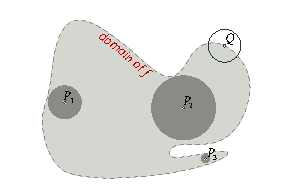
\includegraphics[width=0.6\textwidth]{01domain-is-open.pdf}
  \caption{\textbf{Interior and boundary points in the domain of $f$:} $P_1$,
    $P_2$, or $P_3$ are interior points in the domain. Each of these points is
    the center of a sufficiently small disc that is still contained in the
    domain.  For points such as $Q$, that lie on the edge of the domain, any
    disc centered at $Q$ will ``stick out of the domain,'' no matter how small
    the disc is chosen.  If we talk about the derivative of a function at some
    point in its domain, then, \textit{in this course}, we will always assume
    that we are not at an edge-point like $Q$.}
  \label{fig:domain-is-open}
\end{figure}

The other standing assumption we make in this course is that
\begin{equation}
  \text{\itshape all functions we consider are continuous.}
  \label{eq:all-functions-continuous}
\end{equation}
We have seen the concept of continuity for functions of one variable.  For
functions of more variables ``continuity'' has a similar definition. In this
course we will aim for an intuitive understanding of the concept, which can be
formulated as follows.
\begin{quote}
  \itshape%
  The function $z=f(x, y)$ is continuous at some point $(a,b)$ if the function
  value $f(x, y)$ at any point $(x,y)$ is close to $f(a, b)$ when $(x,y)$ is
  close to $(a,b)$.
\end{quote}
There are many other ways of describing continuity, e.g.~one can say that $f$ is
continuous at $(a,b)$ if
\[
\lim_{(x,y)\to(a,b)} f(x,y) =f(a,b).
\]
To make this precise we would have to define what ``$\lim_{(x,y) \to
  (a,b)}\dots$'' means.

A precise definition of ``$f$ is continuous at $(a,b)$'' invokes $\varepsilon$'s
and $\delta$'s:
\begin{quote}
  \itshape%
  The function $z=f(x, y)$ is continuous at some point $(a,b)$ if for every
  $\varepsilon>0$ there is a $\delta>0$ such that for every point $(x,y)$ that
  lies in the disc of radius $\delta$ centered at $(a,b)$ one has $|f(x,y) -
  f(a,b)| < \varepsilon$.
\end{quote}
In this course we will not use the definition much, but we will occasionally
appeal to the intuitive notion of ``continuity.''  The problems show some
examples of how a function of two variables can fail to be
continuous (e.g.~Problem~\ref{prb:some-discontinuous-functions}).

Now that we have dispensed with these preliminary issues, we can go on to the
central topic in the first half of the semester: partial derivatives and the
chain rule.

\section{Partial Derivatives}        
The derivative $f'(x)$ of a function of one variable, $y=f(x)$, measures a rate
of change: if we increase $x$ by a small amount $\Delta x$ then $y=f(x)$ also
increases by a small amount $\Delta y$.  The ratio between these two changes is
the derivative: $f'(x) \approx \frac{\Delta y}{\Delta x}$.

For a function $z=f(x, y)$ of two variables there is a similar concept: if we
change $x$ and/or $y$ by a small amount then $z$ will also change by a small
amount, and there are formulas relating the changes $\Delta x$, $\Delta y$ and
$\Delta z$.  Because there are many different ways in which we can change $x$
and $y$ there are a few different formulas.  We will encounter the following
versions of ``the derivative of $f(x, y)$'':

\textcolor{badgerred}{$\blacktriangleright$} Change only one of the variables
but not the other: this leads to the so-called \emph{partial derivatives}.

\textcolor{badgerred}{$\blacktriangleright$} Simultaneously vary both $x$ and
$y$: the resulting change turns out to be the sum of the changes we would get if
we were to vary only $x$ or only $y$, respectively.  This will follow from the
\emph{chain rule}, and the resulting formula is called the \emph{total
  derivative}.

We begin with the partial derivatives.

\begin{definition}[Definition of Partial Derivatives]
  If $z=f(x, y)$ is a function of two variables then the partial derivatives of
  $f$ with respect to $x$ and with respect to $y$ are
  \begin{equation}\label{eq:partial-wrt-x-defined}
    \pdd fx(x, y)
    = \lim_{\Delta x\to 0}
    \frac{f(x+\Delta x, y) - f(x, y)}{\Delta x}
  \end{equation}
  and
  \begin{equation}\label{eq:partial-wrt-y-defined}
    \pdd fy(x, y)
    = \lim_{\Delta y\to 0}
    \frac{f(x, y+\Delta y) - f(x, y)}{\Delta y}
  \end{equation}
\end{definition}


\begin{figure}[h]\flushleft
  \def\verticalderivativetext{\dfnt$\dfrac{\partial f}{\partial y}$ is the rate
    of change of $f$ in the vertical direction}
  \def\horizontalderivativetext{\dfnt$\dfrac{\partial f}{\partial x}$ is the
    rate of change of $f$ in the horizontal direction}
  \def\domaintext{\parbox{3in}{\dfnt When we define the partial derivatives at
      some point $(x,y)$, we assume that the function is defined on some
      sufficiently small disc centered at that point $(x,y)$. }} \input
  ../figures/234/02domain-for-partial-derivs.pdf_tex
  \caption{The partial derivatives of a function at some point $(x,y)$ measure
    how fast the function $f(x,y)$ changes if we move the point either
    horizontally (the $x$ direction) or vertically (the $y$ direction).  }
  \label{fig:about-the-partials}
\end{figure}

The following more convenient notation is used very often (because it's so much
shorter):
\begin{equation}
  f_x(x, y) = \pdd fx(x,y),\qquad
  f_y(x, y) = \pdd fy(x,y).
\end{equation}
When we are in a hurry we can also drop the ``$(x, y)$'' from our notation for
derivatives and just write $f_x$ and $f_y$.

\subsection{Partial derivatives of functions of three or more variables} 
If a function depends on three or more variables then one can define its partial
derivatives in the same way as for functions of two variables.  For instance, if
$w=f(x, y, z)$ is a function of three variables, then its partial derivative
with respect to $x$ is defined to be
\[
\pdd fx = \lim_{\Delta x\to0} \frac{f(x+\Delta x, y, z) - f(x, y, z)}{\Delta x}.
\]
The derivatives of $f$ with respect to $y$ and $z$ have very similar
definitions.

\subsection{Examples}
\label{sec:partial-derivatives-examples}
Computing partial derivatives is not harder than computing ordinary derivatives.
To find the partial derivative of a function with respect to $x$ we just pretend
all other variables are constants and differentiate.  Or, in other words, we
could think of the partial derivative of $f(x,y)$ with respect to $x$ as the
ordinary derivative of the function $f$ in which we have frozen the variable $y$
at some particular value.

For instance, the partial derivatives of the function $f(x, y, z) = x^2\sin\pi
y+z$ of \emph{three} variables $x$, $y$, and $z$, are
\[
f_x = 2x\sin\pi y,\quad f_y = \pi x^2\cos\pi y\text{ and } f_z = 1.
\]


\section{Problems}
\label{sec:partial-derivative-problems}
\begin{multicols}{2}
  % \immediate\write\ans{\string\newpage}
\problemfont
\problem \label{prb:some-discontinuous-functions}
For each of the following functions sketch the graph (use a graphing program, if
necessary) and decide if you think the function has a limit as $(x,y)$
approaches $(0,0)$.

\subprob $\DS f(x,y) = \frac{xy}{x^2+y^2}$

\subprob $\DS g(x, y) = \frac{1}{x^2+y^2}$

\subprob $\DS h(x, y) = \frac{x}{x^2+y^2}$.

\subprob $\DS p(x, y) = \frac{x}{\sqrt{x^2+y^2}}$.

\subprob $\DS q(x, y) = \frac{x^2}{\sqrt{x^2+y^2}}$.


\problem\label{prb:01compute-these-partials}
Find the partial derivatives of the following functions:

\subprob 
$\DS f(x,y)=x^2y^3-x^3y^2$.

\subprob 
$\DS f(x,y)=\cos(x^2y)+y^3$.
\answer
$-2xy\sin(x^2y)$, $-x^2\sin(x^2y)+3y^2$
\endanswer

\subprob $\DS f(x,y)={xy\over x^2+y}$.
\answer
$(y^2-x^2y)/(x^2+y)^2$, $x^3/(x^2+y)^2$
\endanswer

\subprob $\DS f(x, t) = (x+t)^4$.

\subprob $\DS f(x, t) = (x-t)^4$.

\subprob $\DS f(x, t) = \sin\omega t \cos\frac{2\pi x}{L}$.

\bigskip

\subprob $\DS f(x,y)=e^{x^2+y^2}$.
\answer
$2xe^{x^2+y^2}$, $2ye^{x^2+y^2}$
\endanswer

\subprob $\DS f(x,y)=xy\ln(xy)$.
\answer
$y\ln(xy)+y$, $x\ln(xy)+x$
\endanswer

\subprob $\DS f(x,y)=\sqrt{1-x^2-y^2}$.
\answer
$-x/\sqrt{1-x^2-y^2}$, $-y/\sqrt{1-x^2-y^2}$
\endanswer

\subprob $\DS f(x, y, z) = \sqrt{x^2 + y^2 + z^2}$

\subprob $\DS f(u,v) = e^{u+v}$

\subprob $\DS f(x,y)=x\tan(y)$.
\answer
$\tan y$, $x/\cos^2 y$
\endanswer

\subprob $\DS f(x,y)={1\over xy}$.
\answer
$-1/(x^2y)$, $-1/(xy^2)$
\endanswer

\problem \label{prb:derivative-of-radius}% 
Let $r$ be the radius in polar coordinates, as defined in
\S~\ref{sec:functions-in-PC} of Chapter III.

\subprob Compute the partial derivatives of $r$.

\subprob Show that the partial derivatives of $r$ can be written as
\[
\pdd rx = \frac xr, \quad
\pdd ry = \frac yr.
\]

\problem \label{prb:derivative-of-theta}% 
Let $\theta$ be the polar angle function, defined in
\S~\ref{sec:functions-in-PC-theta} of Chapter III.

\subprob In the right half plane the function $\theta$ is defined by
\[
\theta(x,y) = \arctan\frac{y} {x}.
\]
Use this expression to find its partial derivatives, $\pdd\theta x$ and $\pdd\theta y$.
\answer
$\DS\pdd\theta x = -\frac{y} {x^2+y^2}$, $\DS\pdd\theta x = \frac{x} {x^2+y^2}$.
\endanswer

\subprob {\tiny\textdbend} Check that the angle function also satisfies
\[
x\sin\theta = y\cos \theta
\]
at all points in the plane.  Use implicit differentiation to find the partial
derivatives $\pdd\theta x$ and $\pdd\theta y$.


\problem Let $f(x, y) = $ the distance from $(x,y)$ to the origin. 
Find a formula for $f$, and compute
\[
f_x, \quad f_y, \text{ and } \sqrt{f_x^2 +f_y^2}.
\]
(Hint: compare this problem with problem \ref{prb:derivative-of-radius}.)
\answer
The distance to the origin is exactly the radius in polar coordinates, so
$f(x, y) = \sqrt{x^2+y^2}$, and
\[
f_x = \frac{x} {\sqrt{x^2+y^2}},\qquad
f_y = \frac{y} {\sqrt{x^2+y^2}}.
\]
This is the same as in problem~\ref{prb:derivative-of-radius}.  The only
quantity that we did not compute before is
\[
\bigl(f_x\bigr)^2 + \bigl(f_y\bigr)^2 = \frac{x^2} {x^2+y^2} + \frac{y^2}
{x^2+y^2} = \frac{x^2+y^2} {x^2+y^2} = 1.
\]
\endanswer

\problem Suppose $f(t)$ and $g(t)$ are single variable differentiable 
functions.  Find $\partial z/\partial x$ and
$\partial z/\partial y$ for each of the following two variable functions.

\subprob  $z=f(x)g(y)$
\answer
$\frac{\pd z}{\pd x} = f'(x)g(y)$, 
$\frac{\pd z}{\pd y} = f(x)g'(y)$.
\endanswer

\subprob  $z=f(xy)$
\answer
$\frac{\pd z}{\pd x} = yf'(xy)$, 
$\frac{\pd z}{\pd y} = xf'(xy)$.
\endanswer

\subprob  $z=f(x/y)$
\answer
$\frac{\pd z}{\pd x} = \frac{1}{y}\, f'(\frac xy)$, 
$\frac{\pd z}{\pd y} = -\frac{x}{y^2} \, f'(\frac xy)$.
\endanswer

\problem
\label{prb:distance-to-square-partialderivs}
Let $f$ be the \emph{distance to the square $Q$ function} from
problem \ref{prb:distance-to-square-level-sets}.  Find the partial
derivatives $f_x$ and $f_y$ of $f$.  (You will need your answer to
problem \ref{prb:distance-to-square-level-sets}, in particular the
description of $f$ as a ``piecewise defined function''.)


\end{multicols}

\section{The linear approximation to a function}
\label{sec:the-linear-approximation-of-a-function}

\subsection{The Chain Rule and friends}     
When we compute the partial derivative of a function with respect to a variable
$x$ we pretend all other variables are constants, and just differentiate with
respect to $x$, just as we would in first semester calculus.  There is therefore
no need to state a product rule or quotient rule, because these are
\textit{exactly the same} as for functions of one variable.  The chain rule on
the other hand is different: there is a chain rule for functions of several
variables, but it has more terms than the chain rule from one-variable calculus.
There are several related topics that fit together in a discussion of the chain
rule, namely \emph{Linear Approximation}, \emph{Tangent Planes to a Graph}, and
\emph{The Total Derivative}.  We will go through these one at a time in the next
few sections.


\subsection{The linear approximation formula}
\label{sec:linear-approximation-no-error}
The key to the chain rule is the linear approximation formula.  This formula
tells us approximately how much a function $z=f(x, y)$ of two variables changes
if both variables are subjected to a small change.

More precisely, if we have a function $z=f(x,y)$, and we know its value
$f(x_0,y_0)$ at some point $(x_0,y_0)$, then how much does the function value
change if $x$ is increased from $x_0$ to $x_0+\Delta x$, and if $y$ is similarly
increased from $y_0$ to $y_0+\Delta y$?
\begin{figure}[h]

  \parbox{0.4\textwidth}{\input ../figures/234/01chainrule.pdf_tex}
  \hfill
  \parbox{0.59\textwidth}{\dfnt%
    We can change $(x_0,y_0)$ to $(x_0+\Delta x, y_0+\Delta y)$ in
    two steps: \\
    \null\quad first keep $y$ fixed and increase $x$ by $\Delta x$,\\
    \null\quad then keep $x$ fixed and increase $y$ by $\Delta y$}
 
  \parbox{0.4\textwidth}{\input ../figures/234/01chainrule-mvt-points.pdf_tex}
  \hfill
  \parbox{0.59\textwidth}{\dfnt%
    To express the change in function values in terms of derivatives, we can use
    the Mean Value Theorem.   We get two intermediate points:\\
    \null\quad one at $x=\tilde x$ for the increase in $f$ when $x$ changes, and\\
    \null\quad one at $y=\tilde y$ for the increase in $f$ when $y$ changes.}
 
  \caption{Computation of the linear approximation
    \eqref{eq:linear-approx-derivation} }
  \label{fig:computation-of-linear-approximation}
  % we compute the change in
  % function value when we go from $(x_0, y_0)$ to $(x_0+\Delta x, y_0+\Delta
  % y)$
  % by adding the change that occurs when we first go from $(x_0, y_0)$ to
  % $(x_0+\Delta x, y_0)$, and then from $(x_0+\Delta x, y_0)$ to $(x_0+\Delta
  % x,
  % y_0+\Delta y)$.
\end{figure}

% The quick version
The basic idea in the computation of the change in $f(x, y)$ is to go from
$(x_0,y_0)$ to $(x_0+\Delta x, y_0+\Delta y)$ in two steps:
\begin{align}
  \label{eq:linear-approx-derivation}
  \Delta f & = f(x_0+\Delta x, y_0+\Delta y) - f(x_0, y_0)\\
  &= \underbrace{f(x_0+\Delta x, y_0+\Delta y) - f(x_0+\Delta x, y_0)}
  _{\text{only $y$ changes}} + \underbrace{f(x_0+\Delta x, y_0) - f(x_0,
    y_0)}_{\text{only $x$ changes}} \nonumber
\end{align}
We have written the total change in $f$ as the sum of two changes, one of them
caused by the change in $x$, and the other due to the change in $y$.  See
Figure~\ref{fig:computation-of-linear-approximation}.

In the second difference only $x$ changes while $y$ remains the same, so we can
use the one variable Mean Value Theorem to conclude that there is some number
$\tilde x$ between $x_0$ and $x_0+\Delta x$ with
\[
\frac{f(x_0+\Delta x, y_0) - f(x_0, y_0)}{\Delta x} = f_x(\tilde x, y_0),
\]
i.e.
\begin{equation}
  f(x_0+\Delta x, y_0) - f(x_0, y_0) = f_x(\tilde x, y_0) \cdot \Delta x.
  \label{eq:change-caused-by-Dx}
\end{equation}
Likewise, in the difference in \eqref{eq:linear-approx-derivation} where only
$y$ changes we can use the Mean Value Theorem to conclude that there is some
$\tilde y$ between $y_0$ and $y_0+\Delta y$ such that
\[
\frac{f(x_0+\Delta x, y_0+\Delta y) - f(x_0+\Delta x, y_0)}{\Delta y} =
f_y(x_0+\Delta x, \tilde y),
\]
and hence
\begin{equation}
  f(x_0+\Delta x, y_0+\Delta y) - f(x_0+\Delta x, y_0) 
  = f_y(x_0+\Delta x, \tilde y) \cdot \Delta y.
  \label{eq:change-caused-by-Dy}
\end{equation}
If we now combine \eqref{eq:change-caused-by-Dx} and
\eqref{eq:change-caused-by-Dy} with \eqref{eq:linear-approx-derivation} then we
get
\[
\Delta f = f_x(\tilde x, y_0)\cdot\Delta x + f_y(x_0+\Delta x,\tilde
y)\cdot\Delta y.
\]
This equation is exactly true, i.e.~we have not made any approximations, and we
have not ignored any kind of ``error terms.''  However, the equation does
contain the numbers $\tilde x$ and $\tilde y$, which are provided by the Mean
Value Theorem, and of which we therefore do not know anything besides the fact
that $\tilde{x}$ lies between $x_0$ and $x_0 + \Delta x$, and $\tilde{y}$ lies
between $y_0$ and $y_0+\Delta y$.  We can get rid of this uncertainty by
settling for an approximation for $\Delta f$ instead of the exact expression we
have just found.  To do this we assume that $\Delta x$ and $\Delta y$ are
``small.''  Then, since $\tilde{x}$ lies between $x_0$ and $x_0+\Delta x$, we
know that $\tilde x\approx x_0$.  We also know that $y_0+\Delta y \approx y_0$,
so, if the function $f_x$ is continuous, then it seems reasonable to assume that
\begin{equation}
  f_x(\tilde{x}, y_0+\Delta y) \approx f_x(x_0, y_0).
  \label{eq:fx-continuous}
\end{equation}
Similarly, we will assume that
\begin{equation}
  f_y(x_0, \tilde{y}) \approx f_y(x_0, y_0).
  \label{eq:fy-continuous}
\end{equation}
Substituting this in \eqref{eq:linear-approx-derivation} we find
\begin{equation}
  \Delta f \approx f_x(x_0, y_0)\Delta x + f_y(x_0, y_0) \Delta y
  \label{eq:linear-approximation-no-error-Deltaf}
\end{equation}
Keeping in mind that $\Delta f = f(x_0+ \Delta x, y_0+\Delta y)-f(x_0,y_0)$, we
conclude
\begin{equation}
  \label{eq:linear-approximation-no-error}
  f(x_0+\Delta x, y_0+\Delta y)
  \approx
  f(x_0, y_0)+f_x(x_0, y_0)\Delta x + f_y(x_0, y_0) \Delta y
\end{equation}

The linear approximation formula \eqref{eq:linear-approximation-no-error} is
often written using Leibniz-style notation for the derivatives, where one writes
$\pdd fx$ for $f_x$, and $\pdd fy$ for $f_y$.  In this notation the
approximation formula takes these forms:
\[
f(x_0+\Delta x, y_0+\Delta y) \approx f(x_0, y_0) + \pdd fx(x_0, y_0)\cdot
\Delta x + \pdd fy(x_0, y_0)\cdot \Delta y,
\]
or, shorter,
\begin{equation}
  \Delta f \approx \pdd fx \Delta x + \pdd fy \Delta y.
  \label{eq:linear-approximation-Leibniz-notation}
\end{equation}

The approximation \eqref{eq:linear-approximation-no-error} can also be written
without $\Delta x$ and $\Delta y$ by a change of notation.  To do this we
introduce
\begin{equation}
  x = x_0 + \Delta x  \text{ and } y = y_0 + \Delta y,
  \label{eq:dxdy-and-xx0-yy0-relation}
\end{equation}
and interpret \eqref{eq:linear-approximation-no-error} as a formula that tells
us approximately what the function value at $(x,y)$ is, provided $(x,y)$ is
close enought to $(x_0,y_0)$.  Written in terms of $x$ and $y$,
\eqref{eq:linear-approximation-no-error} says
\begin{equation}
  f(x,y)
  \approx
  f(x_0, y_0)+f_x(x_0, y_0)\, (x-x_0) + f_y(x_0, y_0) \, (y-y_0).
  \label{eq:linear-approximation-no-error-no-dxdy}
\end{equation}

\subsection{Linear approximation -- infinitesimal version}
\label{sec:linear-approximation-infinitesimal}
We expect the approximation in \eqref{eq:linear-approximation-Leibniz-notation}
to improve as we decrease $\Delta x$ and $\Delta y$ (and we will try to make
this statement more precise in the next section,
\S~\ref{sec:linear-approximation-with-error}).  We could then say, as is
commonly done, that there is an exact equation when $\Delta x$ and $\Delta y$
are ``infinitely small,'' and write this equation as
\begin{equation}
  \label{eq:linear-approximation-infinitesimal}
  df = \pdd fx dx + \pdd fy dy.
\end{equation}
The meaning of this equation is that infinitesimally small changes in $x$ and
$y$, of magnitudes $dx$ and $dy$, respectively, lead to an infinitesimally small
change in $f$ of magnitude $df$, and that $df$, $dx$, and $dy$ are related by
\eqref{eq:linear-approximation-infinitesimal}.  Even though it is very difficult
to make sense of the ``infinitely small'' quantities $dx, dy, df$, in
\eqref{eq:linear-approximation-infinitesimal}, this notation is widely used,
because the make-belief it entails allows one to ignore the more awkward error
terms that we will now discuss.



\subsection{The linear approximation formula with error term}
\label{sec:linear-approximation-with-error}%
In our computation of the change $\Delta f$ of the function we approximated
$f_x(\tilde{x}, y_0)$ by $f_x(x_0, y_0)$, and $f_y(x_0+\Delta x, \tilde{y})$ by
$f_y(x_0, y_0)$.  As a result our linear approximation formula
\eqref{eq:linear-approximation-no-error} is not an exact equation, but only says
that one thing is ``approximately equal'' to another.

We can make this a bit more precise by including error terms, i.e.~by saying
that there are small numbers $e_x$ and $e_y$ such that
\[
f_x(\tilde{x}, y_0) = f_x(x_0, y_0) + e_x, \text{ and } f_y(x_0+\Delta x,
\tilde{y}) = f_y(x_0, y_0) + e_y.
\]
Here $e_x$ and $e_y$ depend on $\Delta x$ and $\Delta y$, and as both $\Delta x$
and $\Delta y$ go to zero, the errors $e_x$ and $e_y$ will also go to zero.

Putting this in \eqref{eq:linear-approx-derivation} we get the linear
approximation formula with error terms:
\begin{multline}
  \label{eq:linear-approximation-with-error}
  f(x_0+\Delta x, y_0+\Delta y) = \underbrace{f(x_0, y_0)+f_x(x_0, y_0)\Delta x
    + f_y(x_0, y_0) \Delta y}_{\text{linear approximation}}\\
  + \underbrace{e_x\Delta x + e_y \Delta y}_{\text{error}}
\end{multline}
in which $e_x$ and $e_y$ depend on $\Delta x, \Delta y$, and satisfy
\[
\lim_{\Delta x, \Delta y \to 0} e_x = \lim_{\Delta x, \Delta y \to 0} e_y = 0.
\]
If we ignore the ``error term'' then we recover the linear approximation
formula~\eqref{eq:linear-approximation-no-error}.  Our more precise linear
approximation formula~\eqref{eq:linear-approximation-with-error} tells us that
the error in \eqref{eq:linear-approximation-no-error} (difference between left
and right hand sides) is given by $e_x\Delta x+ e_y \Delta y$, and that this
error is ``small '' compared to $\Delta x$ and $\Delta y$.  We could write this
as
\[
\text{Error in the approximation} = e_x\Delta x+ e_y \Delta y = o(\Delta x) +
o(\Delta y).
\]



\section{The tangent plane to a graph}\label{sec:the-tangent-plane}
\subsection{The tangent plane}
For a function $z=f(x,y)$ and a point $(x_0,y_0)$ the linear approximation
\eqref{eq:linear-approximation-no-error-no-dxdy} gives us an approximation for
the function $f$ at any other point $(x,y)$ near $(x_0,y_0)$.  It says
\[
z \approx f(x_0, y_0) + f_x(x_0, y_0) (x-x_0) + f_y(x_0, y_0) (y-y_0).
\]
If we replace ``$\approx$'' by equality, then we get a new function of $(x,y)$:
\begin{equation}
  z = f(x_0, y_0) + f_x(x_0, y_0) (x-x_0) + f_y(x_0, y_0) (y-y_0).
  \label{eq:tangent-plane}
\end{equation}
Keeping in mind that $f(x_0, y_0)$, $f_x(x_0, y_0)$, and $f_y(x_0, y_0)$ are
constants, while only $(x,y)$ are variables here, we see that this is the
equation for a plane which we call the \emph{tangent plane} to the graph of $f$
at the point $(x_0, y_0, f(x_0, y_0))$.

\begin{figure}[t]
  \begin{center}
    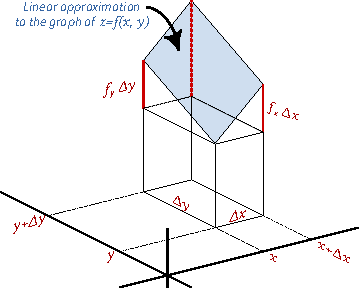
\includegraphics{01totaldifferential.pdf}
    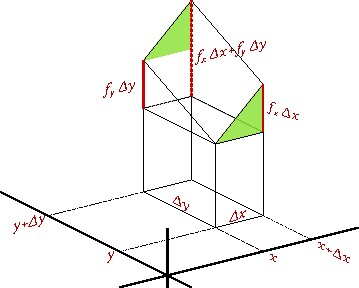
\includegraphics{01totaldifferential-no-tangentplane.pdf}
    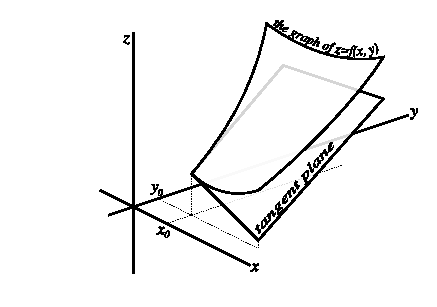
\includegraphics{01tangentplane.pdf}
  \end{center}
  \caption{\textbf{Top: } The graph of the linear approximation of $f$ (graph of
    $f$ itself is not shown -- see the bottom figure).  If we increase $x$ by
    $\Delta x$, then $f$ will increase by approximately $f_x \Delta x$, and if
    we increase $y$ by $\Delta y$, then $f$ increases by approximately $f_y
    \Delta y$.  If we increase $x$ and $y$ by $\Delta x$ and $\Delta y$ at the
    same time, then $f$ increases by roughly $f_x\Delta x+f_y \Delta y$. The
    vertical dotted line behind
    the parallelogram represents this increase in $f$.\\
    \null\quad\textbf{Bottom: } The graph of a function, and of its tangent
    plane at some point $(x_0, y_0, z_0)$. The tangent plane is the graph of the
    linear approximation to $f$. }
  \label{fig:total-differential-and-tangent-plane}
\end{figure}



\subsection{Example: tangent plane to the saddle surface at the origin}     
\textit{Find the equation for the tangent plane to the saddle surface $z=xy$ at
  the origin.  }

\textit{Solution: } The saddle surface is the graph of the function $f(x, y) =
xy$ whose partial derivatives are $f_x(x, y) = y$ and $f_y(x,y) = x$.  To find
the tangent plane at $x_0=0$, $y_0=0$, we compute the partial derivatives,
\[
f_x(x, y) = \pdd{xy}x = y, \text{ so at $(x_0,y_0) = (0,0)$ we have } f_x(0,0) =
0,
\]
and
\[
f_y(x, y) = \pdd{xy}y = x, \text{ so at $(x_0,y_0) = (0,0)$ we have } f_y(0,0) =
0,
\]
Moreover, we also have $f(x_0,y_0) = f(0,0) = 0$, so that the equation for the
tangent plane is
\[
z= 0 + 0\cdot(x-0) + 0\cdot(y-0) = 0,
\]
i.e.,
\[
z=0.
\]
The tangent plane at the origin is just the $xy$-plane.

\begin{figure}
  \centering
  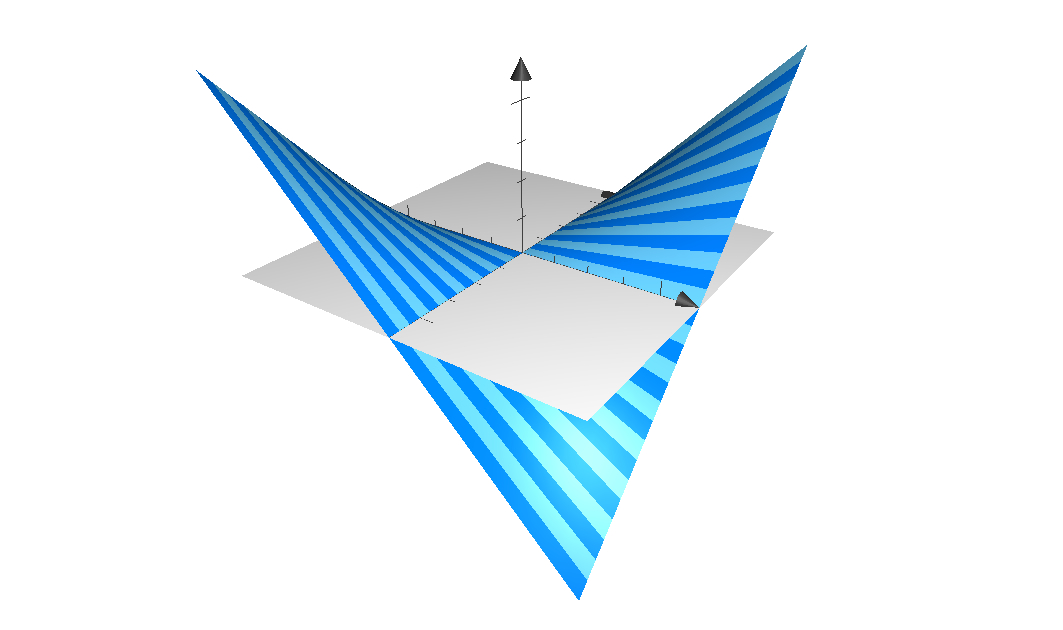
\includegraphics[width=0.7\textwidth]{02saddle-with-tangent.jpg}
  \caption{The graph of $z=xy$ and the tangent plane at the origin. }
  \label{fig:saddle-with-tangent}
\end{figure}

\subsection{Example: another tangent plane to the saddle surface}
\label{sec:another-tangent-to-the-saddle}%
\textit{Find the equation for the tangent plane to the saddle surface $z=xy$ at
  the point $(2,1,2)$.  Where does this plane intersect the coordinate axes?}

\textit{Solution: } This is almost the same problem as before.  The only
difference is that we are trying to find the tangent plane at a point other than
the origin.  To get the tangent plane at the point $(x_0,y_0) = (2,1)$ we
compute the derivatives
\[
f_x(x,y) = y \implies f_x(2,1) = 1,
\]
and
\[
f_y(x, y) = x \implies f_y(2,1) = 2.
\]
The equation for the tangent plane is therefore
\begin{align}
  \label{eq:tangent-to-saddle}
  z &= x_0y_0 + y_0(x-x_0) + x_0(y-y_0)\\
  &= 2+1\cdot(x-2)+2\cdot(y-1) \nonumber\\
  &= -2 +x +2y \nonumber
\end{align}
The intersections with the $x$, $y$ and $z$ axes are, respectively, $(2,0,0)$,
$(0,1,0)$, and $(0,0,-2)$.

\subsection{Example: tangent plane to a sphere}
\label{sec:tangent-plane-to-sphere-as-graph}%
\textit{The point $(x_0, y_0, z_0)$ lies on the upper half of the sphere with
  radius 4 centered at the origin.  Find an equation for the tangent plane to
  the sphere at that point, if $x_0 = 1$ and $y_0=3$.}

  \smallskip

\noindent%
\begin{minipage}{0.48\textwidth}
  \setlength\parindent{16pt}%
  \textit{\color{badgerred}Solution: } The equation for the sphere is
  $x^2+y^2+z^2 = 4^2 = 16$, so the upper half is the graph of the function
  \[
  f(x, y) = \sqrt{16 - x^2 - y^2}.
  \]
  The $z$ coordinate of the given point is therefore $z_0 = \sqrt{16-1^2-3^2} =
  \surd{6}$.  The partial derivatives of $f$ at $(x_0,y_0) = (1,3)$ are
  \begin{align*}
    \pdd fx&= \frac{-x_0}{\sqrt{16 - x_0^2 - y_0^2}} = -\frac{1}{\surd6}, \\
    \pdd fy&= \frac{-y_0}{\sqrt{16 - x_0^2 - y_0^2}} = -\frac{3}{\surd6}.
  \end{align*}
  The equation for the tangent plane is then
  \begin{align*}
    z &= \surd6 - \frac{1}{\surd6}(x-1) - \frac{3}{\surd6}(y-3)\\
    &=\frac{16}{\surd6} - \frac{x}{\surd6} - \frac{3y}{\surd6}.
  \end{align*}
\end{minipage}
\hfill
\begin{minipage}{0.48\textwidth}
  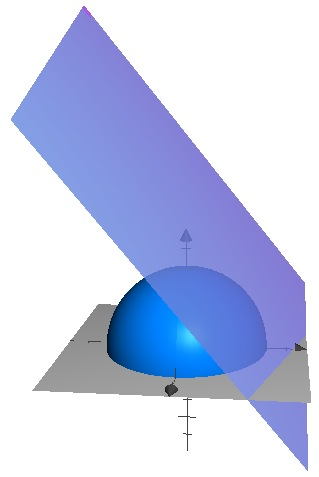
\includegraphics[width=0.8\textwidth]{02sphere-with-tangent.jpg}
\end{minipage}

\section{The Two Variable Chain Rule}
\subsection{The chain rule}
\label{sec:chain-rule-derivation}
Given two functions $x=x(t)$, $y=y(t)$ of one variable, and a function $z=f(x,
y)$ of two variables, then what is the derivative of the function
\[
g(t) = f(x(t), y(t))?
\]
We can find a general formula for $g'(t)$ by using the linear approximation
(\S~\ref{sec:the-linear-approximation-of-a-function}) in the following way.

To find $g'(t_0)$ for some $t_0$, we must compute
\[
\frac{g(t_0 + \Delta t) - g(t_0)}{\Delta t}
\]
and let $\Delta t\to 0$.

If $t$ increases by an amount $\Delta t$ from $t_0$ to $t_0+\Delta t$, then $x$
and $y$ will also change.  We write $\Delta x$ and $\Delta y$ for the changes in
$x$ and $y$, i.e.
\[
\Delta x = x(t_0+\Delta t) - x_0 , \qquad \Delta y = y(t_0+\Delta t) - y_0,
\]
where $x_0 = x(t_0)$ and $y_0=y(t_0)$.  The resulting change in $g$ is thus
\begin{align*}
  \Delta g &= g(t_0+\Delta t) - g(t_0)\\
  &= f\bigl( x(t_0+\Delta t), y(t_0+\Delta t)\bigr) - f\bigl(x(t_0), y(t_0)\bigr) \\
  &= f(x_0+\Delta x, y_0+\Delta y) - f(x_0, y_0).
\end{align*}
By the linear approximation formula \eqref{eq:linear-approximation-with-error}
one then has
\[
\frac{\Delta f}{\Delta t} = f_x(x_0, y_0) \frac{\Delta x}{\Delta t} + f_y(x_0,
y_0) \frac{\Delta y}{\Delta t} + e_x \frac{\Delta x}{\Delta t} + e_y
\frac{\Delta x}{\Delta t}
\]
As we let $\Delta t\to0$ the quotients $\Delta x/\Delta t$ and $\Delta y/\Delta
t$ converge to $x'(t_0)$ and $y'(t_0)$, while the errors $e_x$ and $e_y$
converge to zero, so we get \emph{the two-variable chain rule:}
\begin{equation}
  \label{eq:chain-rule-fxnotation}
  \frac{d f(x(t), y(t))}{dt}
  = f_x(x_0,y_0)\cdot x'(t_0) + f_y(x_0,y_0) \cdot y'(t_0).  
\end{equation}
The chain rule is often also written as
\begin{equation}\label{eq:chain-rule}
  \frac{df}{dt} = \pdd fx \frac{dx}{dt} 
  + \pdd fy  \frac{dy}{dt}.
\end{equation}
This form becomes easy to remember if we interpret the first term as ``the
change in $f$ caused by the change in $x$'' and the second term as ``the change
in $f$ caused by the change in $y$.''

In the way \eqref{eq:chain-rule} is written a number of details are swept under
the rug: the two derivatives $\frac{dx}{dt}$ and $\frac{dy}{dt}$ are ordinary
(Math 221) derivatives of the two functions $x(t)$ and $y(t)$; the two partial
derivatives $\frac{\pd f}{\pd x}$ and $\pdd fy $ are the partial derivatives of
$f$ \emph{in which one has substituted $x(t)$ and $y(t)$.}  A more correct way
of writing the equation would be
\begin{equation}
  \frac{df(x(t), y(t))}{dt}
  = \pdd fx (x(t), y(t)) \cdot x'(t) + \pdd fy (x(t), y(t)) \cdot y'(t).
  \label{eq:chain-rule-Leibniz-verbose}
\end{equation}
Many people find \eqref{eq:chain-rule} easier on the eyes, so that is what we
will usually write.

\subsection{The difference between $d$ and $\pd$}     
Compare \eqref{eq:chain-rule} with the linear approximation formula
\eqref{eq:linear-approximation-infinitesimal} with infinitesimal small
quantities.  Equation \eqref{eq:chain-rule} is just
\eqref{eq:linear-approximation-infinitesimal} in which one has divided both
sides by $dt$.  In contrast to equation
\eqref{eq:linear-approximation-infinitesimal} which contains the strange
``infinitely small quantities'' $dx$, $dy$, $df$, equation \eqref{eq:chain-rule}
contains the derivatives $\frac{dx}{dt}$, etc.\ which \emph{are} well-defined.

Note that we have a breakdown of Leibniz's notation: if we ignore the
distinction between ``$d$'' and ``$\pd$'', and just cancel $dx$ and $\pd x$, and
also $dy$ and $\pd y$ on the right then we end up with
\[
\frac{df}{dt} = \frac{\pd f} {\cancel{\pd x}} \frac{\cancel{dx}} {dt} +
\frac{\pd f} {\cancel{\pd y}} \frac{\cancel{dy}} {dt} = \frac{\pd f}{dt} +
\frac{\pd f}{dt} = 2\frac{\pd f}{dt},
\]
which doesn't make a lot of sense.  The moral: don't cancel $dx$ against $\pd
x$!


\subsection{An example} 
Suppose $x(t) = \cos\omega t$ and $y(t)=\sin \omega t$, so that $\vx(t)=
x(t)\ves1 + y(t)\ves2$ traces out the unit circle.
\begin{center}
  \itshape How fast does $S(t) = 2x(t) + 3y(t)$ change along this motion?
\end{center}
In other words, what can we say about $\frac{dS}{dt}$?

The quantity $S(t)$ is the composition of a function of two variables with the
functions $x(t)$ and $y(t)$, i.e.~it is the result of substituting $x(t)$ and
$y(t)$ in the function $f(x, y) = 2x+3y$.


\subsubsection*{Answer 1 -- without using the chain rule} We can simply compute
\[
  S(t) =2x(t) + y(t) = 2\cos\omega t + 3\sin \omega t 
\]
and differentiate:
\begin{equation}
  \frac{dS}{dt} = \frac{d}{dt}\Bigl\{2\cos \omega t + 3\sin \omega t\Bigr\}
  = -2\omega\sin \omega t + 3\omega \cos\omega t.
  \label{eq:chainrule-example-answer1}
\end{equation}
Note that we did not use our new two-variable chain rule here.  This answer
shows that the point of the two-variable chain rule is not to compute
$\frac{d}{dt}f(x(t), y(t))$ in situations where we have formulas for the
functions $f(x,y)$, $x(t)$, and $y(t)$.  In such a situation we can always
substitute $x(t)$ and $y(t)$ in the function $f(x, y)$ after which we get a
function $S(t) = f(x(t), y(t))$ of one variable.  We learned how to
differentiate those in our first calculus course.

\subsubsection*{Answer 2 -- using the chain rule}
The quantity we want to differentiate is
\[
S(t) = f\bigl(x(t), y(t)\bigr),
\]
where
\[
f(x, y) = 2x+3y, \quad \text{and}\quad x(t) = \cos\omega t, \quad y(t) =
\sin\omega t.
\]
The chain rule tells us that
\begin{equation}
  \frac{dS}{dt} =
  \pdd fx \frac{dx}{dt}  + \pdd fy \frac{dy}{dt}.
  \label{eq:chainrule-example}
\end{equation}
Here the first term stands for the change in $S$ that is caused by the change in
$x$.  To compute it we first find
\[
\pdd fx = \pdd{\{2x+3y\}}x = 2,
\]
so that
\[
\pdd fx \frac{dx}{dt} = 2\cdot \frac{dx}{dt}.
\]
Similarly, the second term in \eqref{eq:chainrule-example} represents the change
in $S(t)$ due to the fact that $y$ is changing:
\[
\pdd fy = \pdd{\{2x+3y\}}y = 3 \implies \pdd fy \frac{dy}{dt} = 3\cdot
\frac{dy}{dt}.
\]
To get the rate of change of $S$ we add both the $x$ and $y$ contributions to
this rate of change, which leads us to
\begin{equation}
  \label{eq:chainrule-example-intermediate-result}
  \frac{dS}{dt} =  2\cdot \frac{dx}{dt} + 3\cdot \frac{dy}{dt}.
\end{equation}
So far we have not used what we know about $x(t)$ and $y(t)$.  This expression
we have just derived for $dS/dt$ is true no matter which $x(t)$, $y(t)$ we are
given.  In our case we have
\begin{align*}
  x(t) &= \cos \omega t \implies \frac{dx}{dt} = -\omega \sin \omega t,\\
  y(t) &= \sin \omega t \implies \frac{dy}{dt} = +\omega \cos \omega t.
\end{align*}
Substitute this in \eqref{eq:chainrule-example-intermediate-result}:
\[
\frac{dS}{dt} = -2\omega\sin \omega t + 3\cos \omega t,
\]
as before.

\subsubsection*{The moral:}
In this example the answer using the chain rule was longer, much more verbose,
and perhaps more complicated than the straightforward computation that led to
our first answer \eqref{eq:chainrule-example-answer1}.  Indeed, if the
derivative of $S$ is all we want then our first computation is the most
efficient way of getting $dS/dt$.  However, the computation using the chain rule
did give us some useful intermediate results, such as the general expression
\eqref{eq:chainrule-example-intermediate-result} for $dS/dt$.  This expression
remains valid if we change the path $(x(t), y(t))$ and can therefore be useful
in situations where, for example, we are allowed to choose the path and we would
like to choose a path for which $dS/dt$ has some prescribed value (e.g.~suppose
we want to keep $S$ constant, how do we choose the path?)

\subsection{Another example} 
Suppose the temperature at the point $(x,y)$ in the plane is given by $T(x, y)$,
and suppose that an ant is walking along the parametrized curve
\[
x(t) = R\cos \omega t, \quad y(t) = R\sin \omega t.
\]
Thus the ant is walking on a circle with radius $R$, and with angular velocity
$\omega$.
\begin{center}\itshape
  How fast is the temperature of the ant changing?\\
  i.e.~compute $\frac{dT}{dt}$.
\end{center}
Here we are not given an explicit formula for the function $T(x,y)$, so we
cannot substitute $x(t)$ and $y(t)$ in $T$ and differentiate using only our
first semester calculus skills.  The approach in Answer 1 of our previous
example does not apply here; we must use the chain rule.

\begin{figure}[h]
  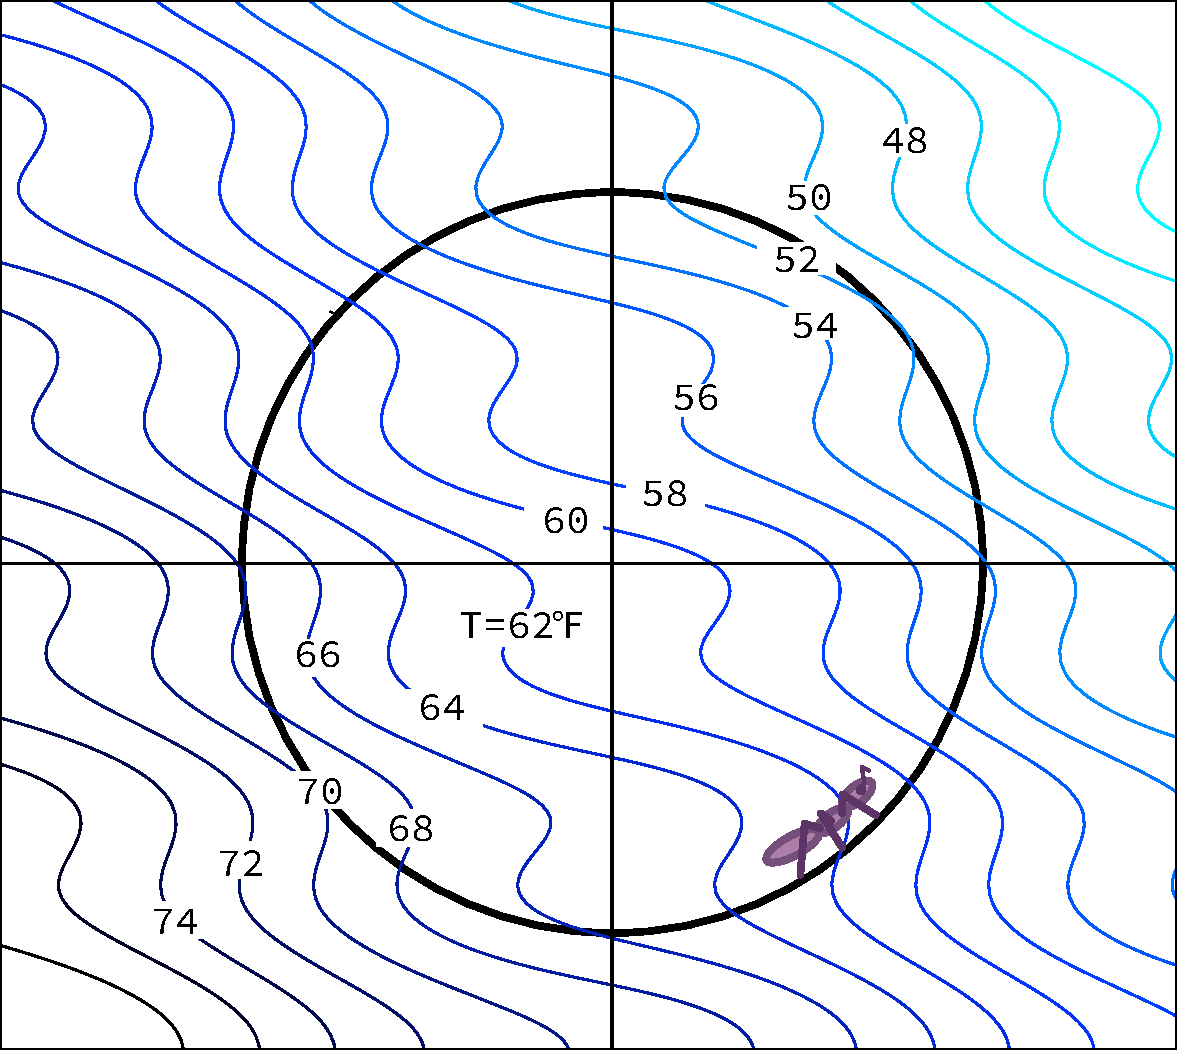
\includegraphics[width=0.5\textwidth]{temperature-of-ant.pdf}
  \caption{Ant walking in a region of varying temperature.}
  \label{fig:temperature-of-ant}
\end{figure}
In \S~\ref{sec:chain-rule-derivation} we have seen several equivalent ways of
writing the chain rule.  Let us look at two of these and consider the meaning of
the terms that arise.

The short form \eqref{eq:chain-rule} of the chain rule tells us that
\[
\frac{dT}{dt} = \pdd Tx \frac{dx}{dt} + \pdd Ty \frac{dy}{dt}.
\]
The $T$ on the left stands for $T(x(t), y(t))$, which we can interpret as the
temperature at the point $(x(t), y(t))$.  That point is the location of the ant
at time $t$, so the $T$ on the left is the temperature the ant feels at time
$t$.  This is a function of $t$.  In mathematical terms it is the result of
substituting (composing) the functions $x(t)$ and $y(t)$ in the function
$T=T(x,y)$.

The two $T$'s on the right appear in partial derivatives.  Here $\pdd Tx$ stands
for the partial derivative of the function $T=T(x, y)$ with respect to the
variable $x$.  One can compute this without knowing the ant's path $(x(t),
y(t))$.  Similarly, $\pdd Ty$ is the partial derivative of $T$ with respect to
$y$.  The partial derivatives $\pdd Tx$ and $\pdd Ty$ themselves are again
functions of $x$ and $y$.  \textit{After} computing these partials they are
meant to be evaluated at the point $(x(t), y(t))$.

This leads us to the more verbose version \eqref{eq:chain-rule-Leibniz-verbose}
of the chain rule, which tells us
\[
\frac{dT(x(t), y(t))}{dt} = \pdd Tx(x(t), y(t))\cdot x'(t) + \pdd Ty(x(t),
y(t))\cdot y'(t).
\]
At this point the only additional information we have is about the ant's motion,
namely, $x(t) = R\cos\omega t$ and $y(t) = \sin \omega t$.  We can compute the
derivatives of $x(t)$ and $y(t)$, which gives us the velocity of the ant in the
$x$ and $y$ directions:
\[
x'(t) = -\omega R\sin \omega t, \qquad y'(t) = \omega R\cos\omega t.
\]
If we substitute everything we know in the chain rule we find that the rate at
which the ant's temperature changes is
\[
\frac{dT}{dt} = -\pdd Tx(R\cos \omega t, R\sin\omega t)\cdot \omega R\sin \omega
t + \pdd Ty(R\cos \omega t, R\sin\omega t)\cdot \omega R \cos\omega t.
\]
To make the equation more readable one can leave out the $(R\cos \omega t,
R\sin\omega t)$, which results in
\[
\frac{dT}{dt} = -\omega R\sin \omega t\pdd Tx + \omega R \cos\omega t\pdd Ty .
\]
The disadvantage of this shorter version is that the reader has to figure out
where we intended to evaluate the two partial derivatives $\pdd Tx$ and $\pdd
Ty$.

\section{Problems}
\begin{multicols}{2}\problemfont

\problem Find the linear approximation to $f(x, y)$ at the point 
$(a,b)$ in the following cases:

\subprob $f(x, y) = xy^2$, $(a, b) = (3,1)$.
\answer
The linear approximation formula is equation
\eqref{eq:linear-approximation-no-error}, in which $x_0 = a = 3$,
$y_0 = b= 1$, and $\Delta x = x-a = x-3$, $\Delta y = y-b = y-1$.  So
for this problem the linear approximation of $f(x,y) = xy^2$ at
$(3,1)$ is
\[
f(x, y) \approx 3 + (x-3) + 6 (y-1) = x+6y-6.
\]
This approximation is only expected to be good when $(x,y)$ is close
to $(3,1)$.  The approximation contains an error which is small
compared to $|x-3|$ and $|y-1|$. 

\noindent
\textbf{FAQ:} What is the relation between the linear approximation
and the tangent plane?

\noindent\textit{Answer:} They are very closely related: the tangent
plane is the graph of the linear approximation. The linear
approximation is the equation for the tangent plane.  To compute
either you have to do the same thing.

\endanswer

\subprob $f(x, y) = x/y^2$, $(a, b) = (3,1)$.
\answer
$x/y^2 \approx 3 + (x-3) - 6 (y-1) = x-6y+6$ when $x$ is close to $3$
and $y$ is close to $1$.
\endanswer

\subprob $f(x, y) = \sin x+ \cos y$, $(a, b) = (\pi,\pi)$.
\answer
$\sin x + \cos y \approx -1 + (-1)(x-\pi) + (0)(y-\pi) = \pi-1-x$ when
$x$ is close to $\pi$ and $y$ is close to $\pi$.
\endanswer


\subprob $f(x, y) = xy/(x+y)$, $(a, b) = (3,1)$.
\answer
$\frac{xy}{x+y} \approx \frac34 + \frac{1}{16}(x-3) + \frac 9 {16}(y-1)$
 when $x$ is close to $3$ and $y$ is close to $1$.
\endanswer

\problem Find an equation for the plane tangent to the graph of $\DS 
f(x,y)=\sin(xy)$ at $(\pi,1/2,1)$. 
\answer
$z=1$
\endanswer

\problem Find an equation for the plane tangent to the graph of $\DS 
f(x,y)=x^2+y^3$ at $(3,1,10)$. 
\answer
$z=6(x-3)+3(y-1)+10$
\endanswer

\problem Find an equation for the plane tangent to the graph of $\DS 
f(x,y)=x\ln(xy)$ at $(2,1/2,0)$. 
\label{prb:ln-tan-plane}
\answer
$z=(x-2)+4(y-1/2)$
\endanswer

% \problem \subprob Find an equation for the tangent plane to the graph of $f(x,
% y) = x^2-2xy$ at the point with $x=2$, $y=1$.

% Find the intersection of the graph of $f$ and the tangent plane you found.
% Show that it consists of two lines.  (Hint: compare with the example in
% \S\ref{sec:01intersect-tangent-with-graph}).  \answer
% % REWRITE THIS
% The graph has equation $z=x^2-2xy$, The tangent plane has equation $z=2x-4y$.

% The part of the tangent plane which lies under the graph is given by
% \[
% 2x-4y < x^2-2xy,
% \]
% i.e.\ by
% \[
% x^2-2xy-2x+4y >0
% \]
% With some luck you see that the LHS can be factored as
% \[
% x^2-2xy-2x+4y = (x-2)(x-2y),
% \]
% so that the part of the tangent plane which is under the graph consists of
% those points $(x,y)$ for which either
% \[
% x>2, \text{ and } x>2y
% \]
% or
% \[
% x<2, \text{ and } x<2y
% \]
% holds.

% The tangent plane and graph intersect along the lines $x=2$ and $x=2y$.
% \begin{center}
%   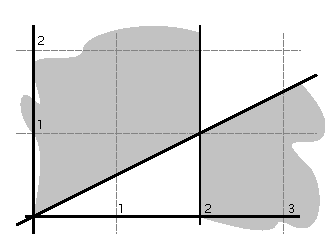
\includegraphics{tangent-below-quadric.pdf}
% \end{center}

% \endanswer

\problem\subprob\label{prb:not-implicit-yet}
Find an equation for the plane tangent to the surface defined by $\DS
2x^2+3y^2-z^2=4$ at $(1,1,-1)$.  (Hint: first write the surface as a graph
$z=f(x, y)$).
\answer
Solve for $z$: $z=\pm\sqrt{2x^2+3y^2-4}$.  In this problem we are
looking at the point $(1,1,-1)$ so we have the graph of $z=f(x,y) = -
\sqrt{2x^2+3y^2-4}$.  The partials are 
\[
\pdd fx = \frac{-2x}{\sqrt{2x^2+3y^2-4}},\qquad
\pdd fy = \frac{-3y}{\sqrt{2x^2+3y^2-4}}
\]
so that, at $(1,1,-1)$ you get $f_x = -2$, $f_y = -3$.  There for the
equation for the tangent plane is $z=-2(x-1)-3(y-1)-1$
\endanswer

\subprob The same question at the point $(1,1,+1)$.


\problem \subprob Suppose you have computed the two partial 
derivatives of a function $z=f(x_0, y_0)$, and you found $f_x(x_0, y_0) = A$ and
$f_y(x_0, y_0) = B$.  Find a normal vector to the tangent plane of the graph of
$z=f(x, y)$ at $(x_0, y_0, z_0)$.

(Hint: If you know the equation for a plane, then how do you find a normal
vector to this plane?)
\answer
The tangent plane has equation $z= z_0 + A(x-x_0) + B(y-y_0)$.  By
putting the variables $x,y,z$ on one side, and all the constants on
the other, you can write this as
\[
Ax +By - z = Ax_0+By_0-z_0.
\]
This is the equation for a plane whose normal is $\vn = \tvek
A\\B\\-1\ttor$.  Any other multiple of this vector is also a valid
normal to the plane, in particular, $\tvek -A\\-B\\+1\ttor$ is OK.

\endanswer

\subprob Find an equation in vector form for the tangent plane to $\DS
x^2+4y^2=2z$ at $(2,1,4)$.  Also find an equation for the normal line to the
graph at $(2,1,4)$.  (The normal line to the graph of a function at some
point $P$, is the line through $P$ that is perpendicular to the
tangent plane to the graph at $P$.)
\answer
We want a normal to the graph of $z = f(x, y) = \frac{1}{2}x^2 + 2y^2$ at the
point $P$.  By the previous problem a normal is given by $\vn = \tvek f_x(2,1)
\\ f_y(2,1) \\ -1 \ttor = \tvek 2\\4\\-1\ttor$.

A line through $P$ in the direction of $\vn$ is given by $\vr (t)=\tvek
2\\1\\4\ttor+t\tvek 2\\4\\-1\ttor$
\endanswer



\problem Imagine a differentiable function, $f(x,y)$.  Make a good 
drawing of the function $f$ and show how $f_x(a, b)$ and
$f_y(a,b)$ are the slopes of two lines which are tangent to the graph
at $(a,b)$.  Indicate clearly which two lines you mean, and describe
how they are defined.

(Can't think of a nice graph?  Take something like the bottom drawing
in Figure~\ref{fig:total-differential-and-tangent-plane}.)
\answer
Below you see the graph of a function and two (solid) lines
which are tangent to the graph.  On one line you have $x=a$
(hence constant), and its slope is $f_x(a,b)$; on the other you have
$y=b$, and it has slope $f_y(a,b)$. 
\begin{center}
  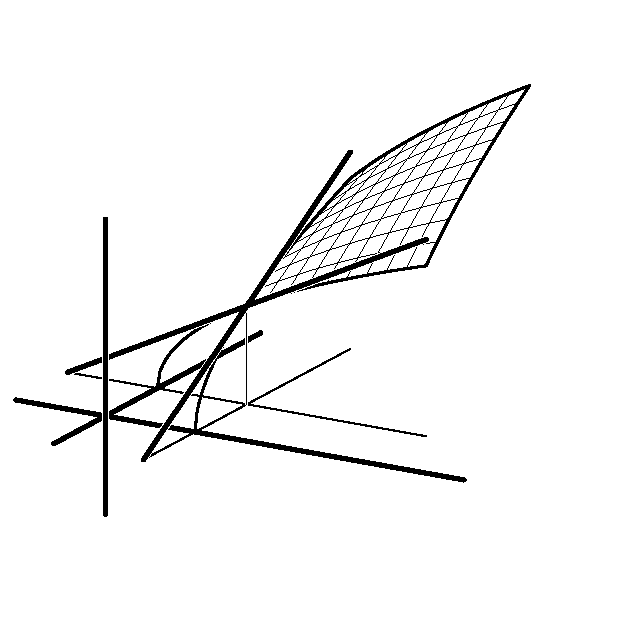
\includegraphics{03two-tangents.pdf}
\end{center}
The tangent plane to the graph (not drawn here, but see
Figure~\ref{fig:total-differential-and-tangent-plane} in the notes)
is the plane containing the two lines in the drawing.
\endanswer

\problem Let $f$ be as in problem~\ref{prb:ln-tan-plane}.  Use linear 
approximation to approximate $f(1.98, 0.4)$ by hand.  Compare your
answer with the actual value of $f(1.98, 0.4)$ (you'll need a
calculator).
\answer
The function is $f(x, y) = x \ln(xy)$.
We have $f(2, \frac{1}{2}) = 2\ln(2\cdot \frac12) = \ln 1 = 0$.
The gradient of the function is $\nab f = \tvek \ln(xy) + 1  \\
x/y\ttor$.
At the point $(2, \frac{1}{2})$ this is $\nab f = \tvek 1 \\ 4\ttor$,
so the linear approximation is 
\[
f(x, y) \approx f(2, \frac{1}{2}) + 1\cdot(x-2)+4\cdot(y-\frac12),
\]
i.e.
\[
f(x, y) \approx 1(x-2) + 4(y-\frac12).
\]
(This is also the answer to problem~\ref{prb:ln-tan-plane}.)

Here we don't want to describe the tangent plan, but we want to find
the value of $f(x, y)$ for $(x,y) = (1.98, 0.4)$.  Substituting these
values of $x$ and $y$ in the linear approximation we get $f(1.98, 0.4)
\approx (1.98-2) + 4 (0.4-0.5) = -0.42$.

This is only an approximation, and you wonder how good it is.  We have
$\Delta x = 1.98-2 = -0.02$, and $\Delta y = 0.4 - \frac12 =
-0.1$\ldots are these numbers ``small''?  To find the error in the
approximation you could use a Lagrange-type remainder term, but that's
not part of math 234.  Instead we grab a calculator and compute
$f(1.98, 0.4) = 1.98\cdot \ln(1.98\cdot 0.4) = -0.46172\cdots$.  So
our linear approximation formula is off by $0.04\cdots$.

\endanswer
\problem
\subprob The tangent plane to the saddle surface $z=xy$ at the origin intersects
the graph of the saddle surface in two lines.  Which lines are they?
\answer
The $x$-and $y$-axes.
\endanswer

\subprob Consider the tangent plane to the saddle surface at $x=2, y=1$
that was computed in \S\ref{sec:another-tangent-to-the-saddle}.  Let $(x,y,z)$
be a point on the saddle surface, and let $(x,y,z_*)$ be the point on the
tangent plane with the same $x$ and $y$ coordinates.  What is the
difference in heights of these two points?
\answer
The heights are the $z$-coordinates, so $z=xy$ and $z_* = -2+x+2y$.  The
difference is
\[
z-z_* = xy - (-2+x+2y) = xy-x-2y+2.
\]
\endanswer

\subprob Show that the saddle surface and its tangent plane intersect when $x=2$
or $y=1$.

\problem
\subprob Find an equation for the tangent) plane to the graph of
$f(x, y) = xy$ at the point $(a, b, ab)$.  Here $a$ and $b$ are
constants which will appear in your answer.
\answer The tangent plane has equation $z=
ab +b(x-a) + a(y-b) = bx+ay-ab$.
\endanswer

\subprob Show that the intersection of the tangent plane and the graph
consists of two straight lines.
\answer The point $(x, y, z)$ lies on the intersection if $z=xy$ and
$z=bx+ay-ab$.  Therefore $x$ and $y$ must satisfy 
$xy-bx-ay+ab = 0$.  This equation factors as follows:
\[
xy-bx-ay+ab = (x-a)(y-b) =0,
\]
so that the intersection contains the line $x=a$, $z=ay$, and
also the line $y=b$, $z=bx$.
\endanswer



\end{multicols}


\section{Gradients}

\subsection{The gradient vector of a function}     
The right hand side in the chain rule \eqref{eq:chain-rule-fxnotation} can be
written as a dot-product of two vectors, namely
\begin{align}
  \label{eq:chainrule-as-dotprod}
  \frac{df}{dt}
  &= f_x(x_0,y_0)\cdot x'(t_0) + f_y(x_0,y_0)\cdot y'(t_0)\\
  &= \vek f_x(x_0, y_0) \\ f_y(x_0, y_0)\tor \dpp \vek x'(t_0) \\
  y'(t_0)\tor\nonumber
\end{align}
This turns out to be so useful that the vector containing the derivatives of $f$
has been given a name.  It is called the \emph{gradient of $f$}, and it is
written as
\begin{equation}
  \nab f(x, y) \stackrel{\sf def}= \vek f_x(x, y) \\ f_y(x, y) \tor
  \label{eq:gradient-defined}
\end{equation}
The symbol $\nab$ is pronounced ``nabla.''

The chain rule, written in vector form, looks like this:
\begin{equation}
  \frac{d f(\vx(t))}{dt} = \nab f(x(t)) \,\dpp\, \vx'(t)
  \label{eq:chainr-rule-vector-form}
\end{equation}
The linear approximation formula \eqref{eq:linear-approximation-no-error} can
also be rewritten more compactly using the gradient vector:
\begin{equation}
  f(\vx_0+\Delta\vx) \approx f(\vx_0) +  \nab f(\vx_0)\,\dpp\, \Delta\vx.
  \label{eq:linear-approximation-vectorform}
\end{equation}
\subsection{The gradient as the ``direction of greatest increase'' for a
  function $f$}
\label{sec:01grad-is-direction-of-greatest-increase}
When we apply the formula
\begin{equation}\label{eq:recall-dot-product}
  \va\dpp\vb = \|\va\|\; \|\vb\|\cos\angle(\va,\vb)
\end{equation}
for the dot product to the vector form
\eqref{eq:linear-approximation-vectorform} of the linear approximation equation,
we find a very useful interpretation of the gradient.  If we are at a point with
position vector $\vx_0$ ($P$ in figure \ref{fig:steepestincrease}) and we are
allowed to make a small step $\Delta \vx$ in any direction we like, but of
prescribed length, then which way should we go if we want to increase $f$ as
much as possible?  And where should we go if, instead, we want to decrease $f$
as much as possible?  What if we want to keep $f$ the same?

\begin{figure}[t]
  \centering \begin{picture} (240.000000,161.967213)(0,0)
    \put(0.0, 0.0){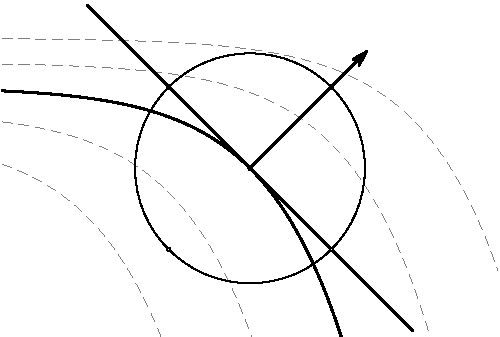
\includegraphics{01steepestdescent.pdf}}
        \put(177.18, 138.16){\sffamily\itshape \makebox[0pt][l]{$\nab f(P)$}}
    \put( -1.05, 117.06){\sffamily\itshape \makebox[0pt][r]{f = 0.0}}
    \put( -1.05,  81.24){\sffamily\itshape \makebox[0pt][r]{-0.6}}
    \put( -1.05, 102.01){\sffamily\itshape \makebox[0pt][r]{-0.3}}
    \put( -1.05, 129.99){\sffamily\itshape \makebox[0pt][r]{0.3}}
    \put( -1.05, 142.15){\sffamily\itshape \makebox[0pt][r]{0.6}}
    \put(154.02, 117.00){\sffamily\itshape \makebox[0pt][r]{$A$}}
    \put( 77.98, 117.00){\sffamily\itshape \makebox[0pt][r]{$B$}}
    \put(159.02,  31.97){\sffamily\itshape \makebox[0pt][c]{$C$}}
    \put( 79.98,  33.97){\sffamily\itshape \makebox[0pt][r]{$D$}}
    \put(117.00,  70.98){\sffamily\itshape \makebox[0pt][r]{$P$}}

\end{picture}

  \caption{The gradient as direction of fastest increase: if we are at a point
    $P$, and we are allowed to jump to any point at a given fixed distance from
    $P$, and if we only know $\nab f(P)$, then the
    linear approximation formula tells us that\\
    \null\quad to maximize $f$ we follow the gradient (choose $A$); \\
    \null\quad to minimize $f$ we go in the direction opposite to
    $\nab f(P)$ (choose $D$); \\
    \null\quad to keep $f$ fixed we move perpendicular to the gradient (choose
    $B$ or $C$).}
  \label{fig:steepestincrease}
\end{figure}

From \eqref{eq:linear-approximation-vectorform} we see that the change in $f$ is
(approximately) given by
\[
\Delta f \stackrel{\rm def}{=} f(\vx +\Delta \vx) - f(\vx)
\stackrel{\textrm{\eqref{eq:linear-approximation-vectorform} } }{\approx} \nab f
\dpp \Delta \vx \stackrel{\text{\eqref{eq:recall-dot-product} }}{=} \|\nab f\|\;
\|\Delta \vx\| \; \cos \theta
\]
where $\theta$ is the angle between the gradient $\nab f$ and the vector $\Delta
\vx$ which represents the step we take.  In this formula the lengths $\nab f$
and $\|\Delta\vx\|$ are fixed, and the angle $\theta$ is the only thing we can
change.  Therefore the largest change in $f$ results if $\cos \theta=+1$, the
smallest when $\cos \theta=-1$, and no change will result if $\cos\theta=0$.  So
we conclude
\begin{itemize}
\item To increase $f$ as much as possible choose $\Delta\vx$ in the direction of
  the gradient $\nab f$,
\item To decrease $f$ as much as possible choose $\Delta\vx$ in the direction
  opposite to the gradient $\nab f$, i.e.\ in the direction of $-\nab f$,
\item To keep $f$ constant choose $\Delta\vx$ perpendicular to the gradient.
\end{itemize}
This is sometimes summarized by saying that \emph{the gradient $\nab f$ points
  in the direction of fastest increase for the function $f$.}

% \begin{equation}
%  \left.\frac{df(\vx + t\vv)}{dt}\right|_{t=0}
%  = \vv\dpp\nab f(\vx)
%  \label{eq:grad-times-vector}
%\end{equation}

%The gradient $\nab f(\vx)$ gives you the direction in which the function $f$
% increases the fastest, since
% \[
% \left.\frac{df(\vx + t\vv)}{dt}\right|_{t=0} = \vv\dpp\nab f(\vx) =
% \bigl\|\nab f(\vx)\bigr\| \, \|\vv\| \,\cos \theta
% \]
% where $\theta$ is the angle between the velocity $\vv$ and the gradient $\nab
% f(\vx)$.

\subsection{The gradient is perpendicular to the level curve}
\label{sec:01gradientperp2levelcurve}
Suppose that for some function $z=f(x,y) $ the level set at level $C$ is a
curve, and suppose that we have a parametric representation $\vx(t) = \tvek
x(t)\\y(t)\ttor$ of this curve.  This means that $x(t)$ and $y(t)$ satisfy
\[
f(x(t), y(t)) = C.
\]
By the chain rule we then get
\[
0= \frac{d f(\vx(t))}{dt} = \nab f(\vx(t)) \dpp \vx'(t),
\]
which tells us that the tangent vector $\vx'(t)$ to the level set is
perpendicular to the gradient $\nab f(\vx(t))$ of the function.  Therefore,
\begin{quote}
  \itshape if $\nab f(x_0,y_0)\neq\vvv0$, then $\nab f(x_0, y_0)$ is a normal
  vector to the tangent to the level curve of $f$ at $(x_0,y_0)$.
\end{quote}
We now have the necessary ingredients to write the equation for the tangent,
namely we know a point $(x_0,y_0)$ on the line, and we know a normal vector to
the line (the gradient).  Thus the equation for the tangent is
\[
\nab f (\vx_0) \dpp (\vx-\vx_0) = 0,
\]
or, equivalently,
\[
\pdd fx(x_0, y_0) \cdot (x-x_0) + \pdd fy(x_0, y_0) \cdot (y-y_0) = 0.
\]
\subsection{The tangent to the parabola $y=x^2$, again}
The very first example anyone sees in their first calculus course must surely be
the computation of the tangent to the parabola $y=x^2$ at the point $(x,y) =
(1,1)$.  We know the answer: it is a line with slope $2$, through the point
$(1,1)$.

We can interpret the parabola as the zero set of the function of two variables
given by $f(x, y) = y-x^2$, and therefore we should be able to find the same
tangent at $(1,1)$ by computing the gradient of $f$.  The computation goes like
this:
\[
f(x,y)=y-x^2 \implies \nab f(x, y) = \vek f_x\\f_y\tor = \vek -2x \\ y\tor.
\]
At $(x,y)= (1,1)$ we have
\[
\nab f(1,1) = \vek -2\\1\tor.
\]%
\marginpar{\centering%
  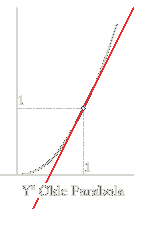
\includegraphics[scale=1.2]{YeOldeparabola.pdf}}%
This vector is perpendicular to the tangent to its zero set.  If we let
$\vx_0=\tvek1\\1\ttor$ be the position vector of our point on the parabola, then
the equation for the tangent to the parabola at this point is
\[
\vn\dpp(\vx-\vx_0) = 0,
\]
i.e.
\[
\vek -2\\1\tor\dpp \vek x-1 \\y-1 \tor = 0.
\]
Simplifying this we get
\[
-2\cdot(x-1) + 1\cdot(y-1)=0, \text{ and thus } y=2x-1.
\]
This is the same line that we found in our first calculus course.

\subsection{Example: the tangent to the zero set of $x^2-y^2+y^3$} 
Consider the zero set of the function
\[
f(x,y) = x^2-y^2+y^3.
\]
The resulting curve is not as familiar as the parabola from the previous
example, and drawing the curve takes some effort\footnote{One could start by
  solving the equation for $x$, which leads to $x=\pm y\sqrt{1-y}$.  This shows
  that $y\leq1$ on the curve.  Graphing $x=y\sqrt{1-y}$ using our 1st semester
  calculus skills then gives us half the curve; the other half is given by its
  reflection in the $y$-axis, i.e.~$x= -y\sqrt{1-y}$. }.

We will not try to draw the whole zero set in this example, but instead we will
see what happens when we try to find the tangent to the zero set at two
different points on the zero set, namely, at $(0,1)$ and at the origin.

\subsubsection*{The tangent at $(0,1)$}
To find the tangent at any point on the zero set of $f$ we use that the normal
to the tangent is given by the gradient of $f$
\[
\nab f = \vek f_x\\f_y\tor =\vek 2x \\ -2y+3y^2\tor.
\]
The normal to the tangent at the point $(0,1)$ is therefore
\[
\vn = \nab f(0,1) = \vek0 \\ -2+3\tor = \vek 0\\1\tor.
\]
In other words, the normal to the tangent at $(0,1)$ is the vertical unit vector
$\ves2$, and therefore the tangent is a horizontal line through $(0,1)$.  Its
equation is $y=1$.  We could also find this equation by working out the general
equation $\vn\dpp(\vx-\vx_0)=0$ for a line with a given normal and point.  Here
we have
\[
\vn = \nab f(0,1) = \vek0\\1\tor, \quad\vx_0 = \vek 0 \\1\tor,
\]
so the equation for the tangent is
\[
\vek0\\1\tor\dpp \vek x-0 \\ y-1\tor = 0,
\]
which simplifies to
\[
y-1=0.
\]

\subsubsection*{The tangent at the origin}
When we repeat the previous calculation at $(x_0, y_0) = (0,0)$ we run into
problems.  These problems begin when we compute the gradient $\nab f$ at the
origin:
\[
\nab f(0,0) = \vek2x \\-2y+3y^2\tor_{x=0, y=0} =\vek 0 \\ 0 \tor.
\]
The gradient at the origin turns out to be the zero vector.  This is problematic
because the zero vector has no direction, and thus is not perpendicular to any
particular line.  \textit{We cannot find the tangent at the origin!}

To see what is going on one has to take a closer look at the curve near the
origin -- see figure~\ref{fig:gradientANDlevels}.  It turns out that near the
origin the zero set of $f$ consists of two smooth curves that cross each
other.\footnote{One way to see this is to solve $x^2-y^2+y^3=0$ for $x$, which
  gives $x=\pm y\sqrt{1-y}$.  Near the origin $y$ is very small, so we can
  approximate $\sqrt{1-y} \approx \sqrt{1}=1$.  The zero set near the origin is
  therefore approximately described by $x=\pm y$, i.e.~two crossing lines.}  The
gradient has to be perpendicular to both of these curves, and the only vector
that achieves this is the zero vector.  Note also that there is no single line
that is tangent to the zero set at the origin.  If we had seen the drawing ahead
of time then we would not have expected to find a tangent to the zero set of $f$
at the origin.

\begin{figure}[ht]
  \begin{center}
    \input ../figures/234/01gradientANDlevels
  \end{center}
  \caption{The zero set of the function $f(x,y) = x^2-y^2+y^3$, and its gradient
    at various points on this zero set.  Since the gradient is always
    perpendicular to the level set of a function, a drawing of the zero set
    tells us the direction of the gradient.  However, the drawing does not say
    anything about the length of the gradient.}
  \label{fig:gradientANDlevels}
\end{figure}


\section{The chain rule and the gradient of a function of three variables}
\subsection{The gradient, etc.}
So far we have only looked at the gradient of a function of two variables.  But
for a function of three variables there is a very similar definition, and the
facts we have discovered have nearly identical counterparts.

If $u=f(x, y, z)$ is a function of three variables, then its gradient is defined
to be the vector
\[
\nab f(x,y,z) = \vek f_x(x, y, z) \\f_y(x, y, z) \\f_z(x, y, z) \tor.
\]
The \emph{chain rule} in this context says that, if $x=x(t)$, $y=y(t)$, and
$z=z(t)$ are functions of one variable, then the derivative of the function we
get by substituting $x(t), y(t), z(t)$ in $f$ is given by any of the following
three equivalent formulas
\begin{align}
  \label{eq:chainrule-threevariables}
  \frac{d f(x(t), y(t), z(t))}{dt}
  &= f_x(x(t), y(t), z(t))\,x'(t) + f_y(x(t), y(t), z(t))\,y'(t)\\
  &\hspace{8em} + f_z(x(t), y(t), z(t))\,z'(t) \nonumber \\[1ex]
  &= \pdd fx \frac{dx}{dt} + \pdd fy \frac{dy}{dt} + \pdd fz \frac{dz}{dt}
  \nonumber\\
  &= \nab f(\vx(t)) \dpp \vx'(t), \text{ where } \vx(t) = \vek
  x(t)\\y(t)\\z(t)\tor.  \nonumber
\end{align}
The linear approximation formula for the function $f$ at some point $(x_0, y_0,
z_0)$, which gives us an approximation of the amount by which $f$ increases if
we go from $(x_0, y_0, z_0)$ to $(x, y, z) = (x_0+\Delta x, y_0 + \Delta y, z_0+
\Delta z)$, is as follows:
\begin{align}
  \label{eq:linearapprox-threevariables}
  \Delta f &=
  f(x, y, z) - f(x_0, y_0, z_0)\\
  &\approx \pdd fx \cdot \Delta x + \pdd fy \cdot \Delta y + \pdd fz \cdot
  \Delta z, \nonumber
\end{align}
in which the partial derivatives are to be evaluated at $(x_0, y_0, z_0)$.
Compare this with the two variable version
\eqref{eq:linear-approximation-no-error-Deltaf}.  In vector form we have
\begin{multline}
  \Delta f = f(\vx_0 + \Delta\vx) - f(\vx_0)
  \approx \nab f(\vx_0) \dpp \Delta\vx,\\
  \text{ where } \vx_0 = \vek x_0\\y_0\\z_0\tor,\; \Delta \vx = \vek \Delta x\\
  \Delta y\\ \Delta x\tor.
  \label{eq:linearapprox-threevariables-vectorform}
\end{multline}
This is the same formula as in the two-variable case, where we had
\eqref{eq:linear-approximation-vectorform}.  The discussion about ``direction of
fastest increase'' applies to the three variable case without change.  Thus, if
we are at a point $\vx_0$, and we are allowed to change our position by a small
vector $\Delta\vx$ of a prescribed length, then we should choose $\Delta\vx$ in
the direction of the gradient $\nab f(\vx)$ if we want to increase $f$ as much
as possible; we should choose $\Delta\vx$ in the direction of $-\nab f(\vx)$ if
we want to \textit{decrease} $f$ as much as possible; and we should choose
$\Delta\vx$ perpendicular to $\nab f(\vx)$ if we want to keep $f$ constant.

\subsection{Tangent plane to a level set}       
If $t=f(x, y, z)$ is a function of three variables then it is hard to visualize
its graph, since this involves drawing \textit{four} mutually perpendicular
axes, something we, three dimensional creatures, cannot do.  However, we can try
to visualize the level sets of the function.  The level set at level $C$
consists, by definition, of all points in three dimensional space whose
coordinates satisfy the equation $f(x, y, z) = C$.

For instance, the unit sphere is given by the equation $x^2+y^2+z^2 = 1$, so it
is the level set at level $1$ of the function $f(x, y, z) = x^2+y^2+z^2$.  The
sphere with radius $R$ is the level set of the same function $f$ at level $R^2$.

Consider a function of three variables, and let $(x_0, y_0, z_0)$ be some point
on the level set at level $C$ (thus $f(x_0, y_0, z_0)=C$.)  The equation for the
level set itself is $f(x,y,z) = C$, and since $(x_0,y_0,z_0)$ satisfies this
equation we can write the equation for the level set as
\[
f(x,y,z) - f(x_0,y_0,z_0) = 0.
\]
Near the point $(x_0,y_0,z_0)$ we can use the linear approximation of $f$ to
approximate the equation for the level set of $f$.  We have
\[
f(x, y, z) - f(x_0, y_0, z_0) \approx \pdd fx \cdot (x-x_0) + \pdd fy \cdot
(y-y_0) + \pdd fz \cdot (z-z_0),
\]
where, as in \eqref{eq:linearapprox-threevariables}, the partial derivatives are
to be computed at the given point $(x_0, y_0, z_0)$.  They are, in particular,
constants (they depend on $(x_0, y_0, z_0)$ but not on $(x, y, z)$.)

\begin{figure}[h]
  \input ../figures/234/tangent-plane-to-levelset.pdf_tex
\end{figure}

Thus we see that near any particular point on the level set of a function we can
approximate the equation for the level set by
\begin{equation}
  \pdd fx \cdot (x-x_0) +
  \pdd fy \cdot (y-y_0) +
  \pdd fz \cdot (z-z_0) = 0.
  \label{eq:levelset-threevars}
\end{equation}
If at least one of the partial derivatives at $(x_0, y_0, z_0)$ is non zero,
then this is the equation of a plane. We call this plane the tangent plane to
the level set.

In vector form the equation for the tangent plane to a level set of $f$ at a
point with position vector $\vx_0$ can be written as
\begin{equation}
  \nab f(\vx_0) \dpp (\vx-\vx_0) = 0.
  \label{eq:levelset-threevars-vectorform}
\end{equation}
From this equation we see that, just as in the case
(\S\ref{sec:01gradientperp2levelcurve}) of level curves of a function of two
variables, \emph{the gradient $\nab f(\vx_0)$ is perpendicular to the tangent
  plane of the level set of the function $f$ at the point $\vx_0$.}

\subsection{Example: tangent plane to a sphere revisited} 
In the example in \S~\ref{sec:tangent-plane-to-sphere-as-graph} we found the
tangent plane to the sphere at the point $(1,3,\sqrt{6})$, where the sphere had
radius $4$, and was centered at the origin.  There we represented the top half
of the sphere as the graph of a function.  We will now redo this calculation by
representing the sphere as the level set of some other function.

By Pythagoras the distance $d$ from a point $(x,y,z)$ to the origin satisfies
\[
d^2 = x^2+y^2+z^2.
\]
The sphere with radius $4$ and center at the origin therefore consists of all
points $(x,y,z)$ that satisfy
\[
x^2+y^2+z^2 = 4^2 = 16.
\]
In other words, it is the level set at level $C=16$ of the function
\[
f(x,y,z) = x^2+y^2+z^2.
\]
To find an equation for the tangent plane through the point $(1,3,\sqrt{6})$ we
need two ingredients: a point on the plane and a normal vector to the plane.
(See Chapter I, \S\ref{sec:defining-eq-planes}.)  We already have a point on the
plane, namely our point $(1,3,\sqrt{6})$, and the normal is given by the
gradient of the function $f$ whose level set is the sphere.  This gradient is
easy to compute.  Since $f(x,y,z) = x^2+y^2+z^2$, we have
\[
\pdd fx = 2x, \quad \pdd fy = 2y, \quad \pdd fz = 2z,
\]
and thus
\[
\nab f (1,3,\sqrt{6}) = \vek 2x \\ 2y \\2z\tor_{ (x,y,z)= (1,3,\sqrt{6}) } =
\vek 2\\ 6\\ 2\sqrt{6}\tor.
\]
The equation for the tangent plane is $\vn\dpp(\vx-\vx_0)=0$, where the normal
$\vn$ to the tangent plane is the gradient $\nab f$ evaluated at our given point
$\vx_0$.  So, the tangent plane is given by
\[
\nab f(1,3,\sqrt6) \dpp (\vx - \vx_0) = 0,
\]
which we can write as
\[
\vek 2\\ 6\\ 2\sqrt{6}\tor \dpp \vek x-1 \\\ y-3 \\ z-\sqrt{6}\tor = 0 ,
\]
i.e.
\[
2(x-1) + 6(y-3) + 2\sqrt{6} (z-\sqrt6) =0.
\]
After some cleaning up we get
\[
x+3y+\sqrt{6} z = 16.
\]
This is the same answer we got in \S\ref{sec:tangent-plane-to-sphere-as-graph}.
\marginpar{
  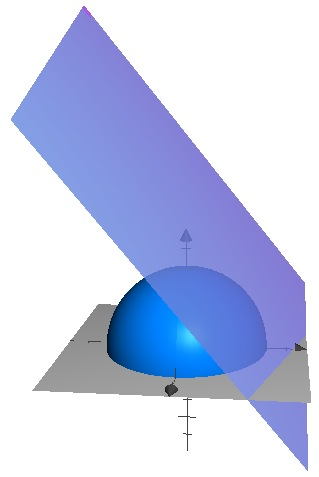
\includegraphics[width=1in]{02sphere-with-tangent.jpg}}

\subsection{Example} \textit{ Find the linear approximation of $F(x, y, z) =
  e^{-y}(x-z)^2$ and tangent plane to its level set at $x=1, y=2, z=5$}
\label{sec:01tangentplane2levelsurface}

\textit{Solution: } At the given values of $x, y, z$ on has $F(1, 2, 5) =
e^{-2}(1-5)^2 = 16/e^2$.  The partial derivatives of $F$ are
\[
F_x = 2(x-z)e^{-y}, \quad F_y = -e^{-y}(x-z)^2, \quad F_z = -2(x-z)e^{-y},
\]
which at $(x, y, z) = (1, 2, 5)$ reduces to $F_x = -8/e^2$, $F_y = -16/e^2$ and
$F_z = +8/e^2$.  If $(x, y, z)$ is close to $(1, 2, 5)$, then the linear
approximation formula tells us that
\[
F(x, y, z) \approx F(1, 2, 5) -\frac8{e^2} (x-1) -\frac{16}{e^2} (y-2) +
\frac8{e^2} (z-5)
\]
or, in ``$\Delta x$'' notation, %
\marginpar{\footnotesize\dfnt%
  By definition:\\
  $\Delta x=x-1$\\
  $\Delta y=y-2$\\
  $\Delta z=z-5$ }
\[
F(1+\Delta x, 2+\Delta y, 5+\Delta z) \approx F(1, 2, 5) -\frac8{e^2} \Delta x
-\frac{16}{e^2} \Delta y + \frac8{e^2} \Delta z.
\]
The equation for the tangent plane to the level set of $F$ at the point
$(1,2,5)$ is therefore
\[
-\frac8{e^2} (x-1) -\frac{16}{e^2} (y-2) + \frac8{e^2} (z-5)=0,
\]
or, after cancelling ${e^2}$'s and $8$'s: $(x-1) + 2(y-2) -(z-5) = 0$.  Further
simplification shows that the equation for the tangent plane is
\[
x+2y-z = 0.
\]

\section{Implicit Functions}
In first semester calculus we learned a procedure for finding derivatives of
implicitly defined functions.  If some function $y=f(x)$ was not given by an
explicit formula, but rather by an implicit equation
\begin{equation}
  F(x, y)=0
  \label{eq:implicit}
\end{equation}
then there was a way to find the derivative of $y=f(x)$ from the above equation
only.  But there was no formula for $f'(x)$.  The reason is that the formula for
the derivative $f'(x)$ involves the partial derivatives of $F$.

In this section we review implicit differentiation again.  The following theorem
is about the zero set of the function $F$.  One usually thinks of the zero set
of a function of two variables as a curve (``an equation defines a curve'') but
this is not always so.  The theorem below gives us a way to find out if the zero
set is really a curve, at least near any given point on the zero set which we
happen to know.

\begin{figure}[ht]
  \centering
  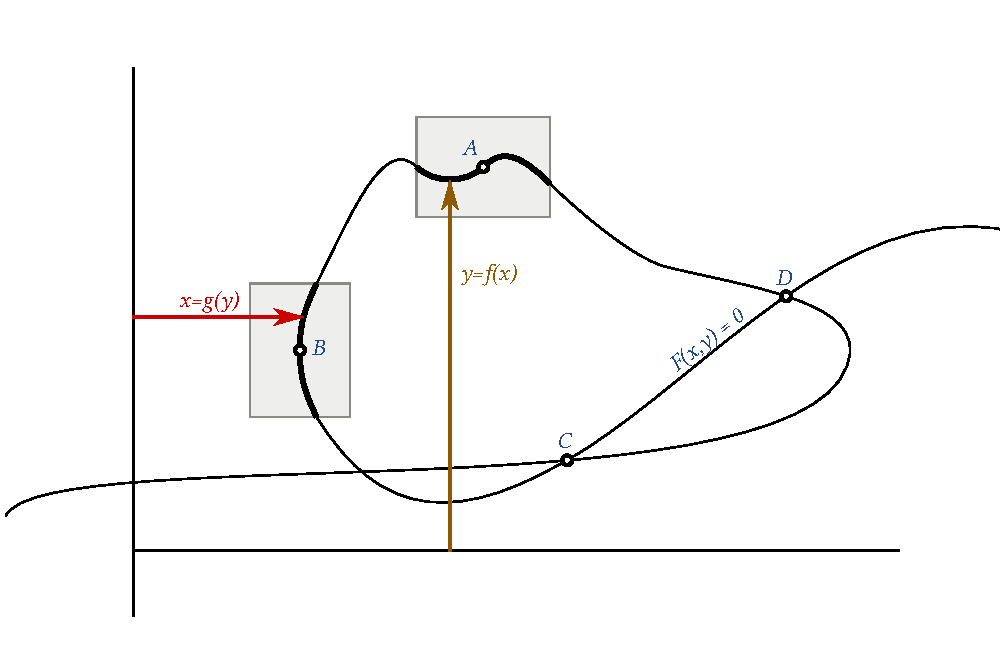
\includegraphics[scale=0.7]{01implicitfunctiontheorem.pdf}
  \caption{ \textbf{The Implicit Function Theorem. } The zero set of a function
    $F(x, y)$ does not have to be the graph of a function, but if at some point
    ($A$) on the zero set we have $F_y\neq0$, then, near that point $A$, the
    zero set is the graph of a function $y=f(x)$.  If $F_x\neq0$ at some point
    ($B$), then near $B$ the zero set is also the graph of a function, provided
    we let $x$ be a function of $y$: $x=g(y)$.\\
    \null\quad\textbf{Exceptional points:} At
    some points, like $C$ and $D$ in this figure, the level set of $F$ cannot be
    represented as the graph of a function $y=f(x)$, nor can it be represented
    as a graph of the type $x=g(y)$.  At such points the Implicit Function
    Theorem implies that both $F_x=0$ and $F_y=0$. }
\end{figure}

\subsection{The Implicit Function Theorem}\itshape
\label{thm:01implicit-function}
Let $F(x, y)$ be a function defined on some plane domain with continuous partial
derivatives in that domain, and suppose that a point $(x_0, y_0)$ in the zero
set of $F$ is given.

If $\pdd Fy (x_0, y_0) \neq 0$ then there is a small rectangle centered at
$(x_0, y_0)$ such that within this rectangle the zero set of $F$ is the graph of
a function $y=f(x)$.  The derivative of this function is
\begin{equation}\label{eq:IFTdydx}
  f'(x) = \frac{dy}{dx} = -\frac{F_x(x, f(x))}{F_y(x,f(x))}.
\end{equation}

If $\pdd Fx (x_0, y_0) \neq 0$ then there is a small rectangle centered at
$(x_0, y_0)$ such that within this rectangle the zero set of $F$ is the graph of
a function $x=g(y)$.  The derivative of this function is
\begin{equation}\label{eq:IFTdxdy}
  g'(y) = \frac{dx}{dy} = -\frac{F_y(g(y), y)}{F_x(g(y),y)}.
\end{equation}


\upshape

A proof may be given in class, time permitting.

There is no need to memorize the formulas \eqref{eq:IFTdydx} and
\eqref{eq:IFTdxdy}.  We can get them by using the method of implicit
differentiation from math 221.  For instance, suppose that the graph of the
function $y=f(x)$ gives you a piece of the zero set of $F$.  This means that
\[
F(x, f(x)) = 0 \text{ for all $x$.}
\]
Differentiating both sides of this equation leads us via the chain rule,
\[
\frac{d F(x, f(x))}{dx} = \pdd Fx (x, f(x)) \cdot \frac{dx}{dx} + \pdd Fy (x,
f(x)) \cdot \frac{df(x)}{dx},
\]
to
\begin{equation}
  0 = \frac{d F(x, f(x))}{dx}
  =F_x(x, f(x)) + F_y(x, f(x)) f'(x).
  \label{eq:IFTdydx-derivation}
\end{equation}
Solve this for $f'(x)$ and we get
\[
f'(x) = \frac{dy}{dx} = -\frac{F_x(x, f(x))}{F_y(x, f(x))},
\]
which is what the theorem claims.

\subsection{The Implicit Function Theorem with more variables}     
There are many variations and extensions of Theorem
\ref{thm:01implicit-function}.  The simplest is to consider the level set of a
function of three rather than two variables.  Suppose $F$ is a function of three
variables, with continuous partial derivatives, and consider the set of points
defined by the equation
\[
F(x, y, z) = C.
\]
This is the level set of $F$ at level $C$.

If
\[
\pdd F y (x_0, y_0, z_0) \neq 0,
\]
then near $(x_0, y_0, z_0)$ the level set of $F$ is the graph of a function
$y=g(x, z)$, meaning that the function $y=g(x, z)$ satisfies
\[
G(x, g(x, z), z) = 0.
\]
Hence we can find the partial derivatives of this function by implicit
differentiation.  The result is
\begin{equation}
  \pdd yx = g_x(x, z) = - \frac{F_x(x, y, z)}{F_y(x, y, z)},\qquad
  \pdd yz = g_z(x, z) = - \frac{F_z(x, y, z)}{F_y(x, y, z)},
  \label{eq:IFTxyz}
\end{equation}
where $y=g(x, z)$.

\subsection{Example -- The saddle surface again}     
The saddle surface is the graph of the function $z=xy$, which we can think of as
the zero set of the function
\[
F(x, y, z) = z- xy.
\]
The point $(2, 3, 6)$ lies on the saddle surface, and at this point the partial
derivatives of $F$ are
\[
F_x =\frac{\pd(z-xy)}{\pd x} = -y = -3, \quad 
F_y =\frac{\pd(z-xy)}{\pd y} = -x = -2, \quad 
F_z =\frac{\pd(z-xy)}{\pd z} = 1.
\]
Since $F_x(2, 3, 6) = -3 $ is non zero, the Implicit Function Theorem tells us
that near this point the zero set of $F$ is the graph of a function $x=g(y, z)$.
Solving $F=0$ for $x$ we see that this function is in fact
\[
x= g(y, z) = \frac{z}{y}.
\]
The partial derivatives of $g$ are easy to compute in this example, but even if
we couldn't find them directly, the Implicit Function Theorem would tell us that
\[
g_y(3, 6) = -\frac{F_y(2, 3, 6)}{F_x(2, 3, 6)} = -\frac{2}{3},\qquad 
g_z(3, 6) = -\frac{F_z(2, 3, 6)}{F_x(2, 3, 6)} = \frac{1}{3}.
\]

\section*{Problems}
\begin{multicols}{2}
\problemfont
\problem Compute the gradient of each function in 
Problem~\ref{prb:01compute-these-partials} of
\S~\ref{sec:partial-derivative-problems}.

\problem\label{prb:prodrule-for-grad} 
Show that for any two differentiable functions $f$ and $g$ one has
\begin{align*}
  \nab(f\pm g) &= \nab f \pm \nab g,\\
  \nab (fg) &= f\nab g+ g\nab f,\\
  \nab \bigl(\frac fg\bigr) &= \frac{g\nab f - f\nab g} {g^2}.
\end{align*}
In other words the sum-, product- and quotient rules for differentiation
also apply to the gradient.
\answer
$\pdd{(f+g)}x = f_x + g_x$, and $\pdd{(f+g)}y = f_y + g_y$, so 
\[
\vek\pdd{(f+g)}x \\ \rule{0pt}{18pt}\pdd{(f+g)}y \tor
= \vek f_x + g_x \\ f_y + g_y\tor
= \vek f_x \\ f_y\tor + \vek g_x \\g_y\tor
\]
Hence $\nab(f+g) = \nab f + \nab g$.

The product and quotient rules follow in the same way.
\endanswer

\problem \subprob Draw the level sets of the function 
$f(x,y) = x^2 + 4y^2$ at levels $0$, $4$, $16$.


\subprob Find the points on the level set $f(x,y) = 4$ where the
gradient is parallel to the vector $\tvek 1\\1\ttor$.  What can you
say about the tangent line to the level set at those points?  Draw the
gradient vectors, and the tangent lines at the points you just found.

\textbf{Hint: } two non-zero vectors $\vv$ and $\vw$ are parallel if
there is a number $s$ such that $\vv = s\vw$.
\answer
The gradient is $\nab f = \tvek 2x \\ 8y\ttor$.  This vector is
parallel to $\tvek1\\1\ttor$ if there is a number $s$ such that
$\nab f = s\tvek1\\1\ttor$, i.e.\ $\tvek f_x \\f_y\ttor  = \tvek
s\\s\ttor$.  This happens if $f_x(x, y) = f_y(x, y)$.  From our
computation of the partial derivatives of $f$ we find that $\nab f$ is
parallel to $\tvek1\\1\ttor$ when $2x=8y$.  This happens at every
point on the line $y=\tfrac14x$. 

We are asked which points on the level set $f=4$ satisfy this
condition, so we must find where the line $y=\frac14x$ intersects the
level set $x^2 + 4y^2 = 4$.  Solving the two equations gives two
points $(\frac45\sqrt{5}, \frac15\sqrt{5})$ and $(-\frac45\sqrt{5},
-\frac15\sqrt{5})$.

\endanswer

\subprob Repeat the same two problems for the function $g(x,y) = 4xy^2$.
\answer
$\nab g = \tvek 4y^2 \\ 8xy\ttor$.  This is parallel to
$\tvek1\\1\ttor$ when $y=2x$.  This line intersects the level set
$g=4$ in the point $(\frac12\sqrt[3]{2},\sqrt[3]{2})$.

\textbf{Note: } when you solve the equations $\nab g = \tvek s\\s\ttor$, you
find $y=2x$, but also the line $y=0$ ($x$-axis).   
On this line the gradient actually vanishes, i.e.\ $\nab g = \vvv0$
and has no direction, so you can't really say it is parallel to
$\tvek1\\1\ttor$.
\endanswer


\problem
\subprob Draw the zero set of the function $f(x, y, z) = x^2+y^2-2z$.
\answer
It's a paraboloid of revolution.  
\endanswer

\subprob Find all points on the zero set of the function $f$ where the
gradient is parallel to the vector $\vv = \tvek1\\1\\2\ttor$.
\answer
$\nab f = \tvek2x\\2y\\-2\ttor = s \tvek1\\1\\2\ttor$ if $-2 = 2s$,
i.e.\ $s=-1$.  This then implies $2x= -1$, $2y = -1$, so that
$x=y=-\frac12$.  Since the point has to lie on the zero set of
$f$, we find $z= \frac12(x^2+y^2) = \frac14$.
\endanswer

\problem A bug is crawling on the surface of a hot plate, the temperature 
of which at the point $x$ units to the right of the lower left corner and
$y$ units up from the lower left corner is given by $T(x,y)=100-x^2-3y^3$.

\subprob If the bug is at the point $(2,1)$, in what direction should it
move to cool off the fastest?  
\answer
At $(2,1)$ the gradient is $\nab T = \tvek -2x \\\ -9y^2\ttor =
\tvek-4 \\ -9\ttor$.  To cool off as fast as possible the bug should
go in the opposite direction, i.e.\ in the direction of $\tvek 4 \\
9\ttor$, or any positive multiple of this vector.

\endanswer

\subprob If the bug is at the point $(1,3)$, in what direction should it
move in order to maintain its temperature?
\answer 
At $(1,3)$ the gradient is $\nab T = \tvek -2 \\ -81\ttor$.
To keep its temperature constant the bug should walk in any direction
perpendicular to the gradient.  The vector $\tvek 81 \\ -2\ttor$ is
perpendicular to the gradient, so the bug should go in the direction
of $\tvek 81 \\ -2\ttor$ or the opposite direction, $\tvek -81 \\ 2\ttor$.

Any non-zero multiple of $\tvek -81 \\ 2\ttor$ is also a valid answer,
since we can only give the \textit{direction} and not the speed.

Remember: the vector $\tvek -b\\a\ttor$ is perpendicular to
$\tvek a\\b\ttor$.

\endanswer



\problem The level sets of a function $z=f(x, y)$ are often curves. 
Must they always be curves? Could the zero set of a function be a
solid square (e.g.\ all points $(x,y)$ with $0\le x\le1$ and
$0\le y\le1$)?
\answer
The zero set doesn't have to be a curve.  For example the zero set of
the function $f(x, y) = $distance from $(x,y)$ to the square
$Q$ (Problems \ref{prb:distance-to-square-level-sets} and
\ref{prb:distance-to-square-partialderivs}) is the whole square $Q$.
\endanswer


\problem The caption of Figure~\ref{fig:gradientANDlevels} says that one can only see the direction, but not the length of the gradient $\nab f$ of a function, from just one of its level sets.  It is however possible to see where the gradient is larger from a drawing of several level sets.  We can read this information from the way in which level sets are more bunched together in some regions than in others.

\begin{center}
  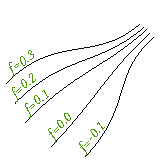
\includegraphics[scale=1.5]{01howBigIsTheGradient.pdf}
\end{center}

The picture above shows some level sets of a function.  On the
bottom left the level sets are further apart, on the top right they
are more bunched together.  Where is the gradient the larger, i.e.~where 
is $\|\nab f\|$ larger: bottom-left, or top-right? 
\answer
$\|\nab f\|$ is larger at the top right, because there the
function $f$ changes faster.
\endanswer

\problem Have a look at Figure~\ref{fig:gradientANDlevels}.  Assume the 
function differentiable at the origin.

\subprob What can you say about the gradient $\nab f$ at the origin?
\answer
The gradient at the origin is the zero vector.  This was explained in the text.
\endanswer

\subprob Where is the function positive and where is it negative
(assume that the whole zero set is drawn).
\answer
The function increases in the direction of the gradient.  Since it vanishes on the curve in Figure~\ref{fig:gradientANDlevels}, the function will be positive in the region above the curve, and it will be negative both below the curve and inside the little loop.
\endanswer

\problem  This problem asks you to think about the Implicit Function Theorem~\ref{thm:01implicit-function}

Consider the unit circle $\setC$ with equation
\[
x^2+y^2=1.
\] 
The unit circle $\setC$ is a level set of the function $F(x,y) = x^2+y^2$.

\subprob Where on $\setC$ is $F_y \neq0$?  Near which points $P$ on $\setC$ can one
represent $\setC$ as a graph of the form $y=f(x)$?

\subprob Near which points $P$ on $\setC$ can one represent $\setC$ as a graph of
the form $x=g(y)$?


\problem  Here is the zero set of a function $z=f(x, y)$ (in bold). 
The function is only zero on the bold curve, it is nonzero everywhere
else.
\begin{center}
  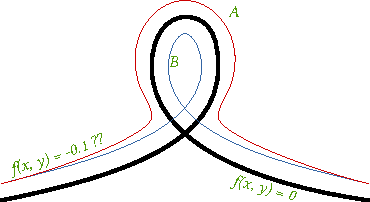
\includegraphics[width=0.4\textwidth]{01LevelSetProblem1.pdf}
\end{center}

\subprob One of the two other curves above is the level set $f(x, y) =
-0.1$.  Which one is it, $A$ or $B$?  As always, explain your answer.

\subprob Draw a possible level set $f(x, y) = +0.1$.

\subprob Draw possible gradients on the zero set (similar to
Figure~\ref{fig:gradientANDlevels}).

\problem Here is the zero set of a differentiable function $z=f(x, y)$. 
\begin{center}
  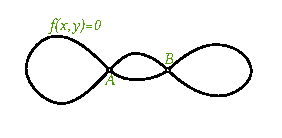
\includegraphics[width=0.4\textwidth]{01findthecriticalpoints.pdf}
\end{center}
Explain why the Implicit Function Theorem (\S
\ref{thm:01implicit-function}) implies that $\nab f=\vvv0$ at the two points
$A$ and $B$.
%
% \subprob Consider the function $g(x, y) = f(x,y)^2$.  Show that $f$ and $g$
% have the same zero set.
%
% \subprob Show that $\nab g = 2f\nab f$.  (Hint: look at problem
% \ref{prb:prodrule-for-grad}).
%
% \subprob Show that $\nab g=\vvv0$ at \emph{all} points on the zero set of $g$.
%
\problem \subprob Compute the gradient of the ``distance to the square 
function'' $f$ from problems \ref{prb:distance-to-square-level-sets}
and \ref{prb:distance-to-square-partialderivs}.

\subprob How much is $|\nab f|$?
\answer
The result of a rather long calculation is that $\|\nab f\| =1$ everywhere outside the 
square, and $\|\nab f\| = 0$ inside the square
(because $f$ is constant in the square.)
\endanswer

\subprob  Make a drawing of the level sets of $f$, and the gradient
$\nab f$.



\problem Let $f(x, y) = \ln(2+2x+e^y)$. 

\subprob Compute the gradient of $f$ at the point $(x_0, y_0)$ with
position vector $\vx_0 = \tvek 1 \\ 0\ttor$.  

\subprob You are allowed to choose a point at a distance $0.01$ from
the point $(1,0)$.  Where would you choose the new point if you want
$f$ to be as large as possible?  (Hint:  review the linear
approximation formula and subsequent discussion about the gradient as
direction of greatest increase in
\S\ref{sec:01grad-is-direction-of-greatest-increase})

\subprob Is your answer to the previous the \textit{exact} answer, or only an
\textit{approximation}?  I.e.,\ could someone else find a point at distance
$0.01$ from $(1,0)$ at which $f$ has a (slightly) higher value than at
the point you found?

\subprob The level set $C$ of $f$ through the point $(1,0)$ happens to be the
graph of a function $y=g(x)$.  Find that function.

\subprob Find a normal vector to the tangent line to $C$ at the point
$(1,0)$.  Find an equation for the tangent line to $C$ at $(1,0)$.  

\subprob How much is $g(1)$?  Find two different ways to compute
$g'(1)$ based on the work you have done so far.


\problem Let $(a,b,c)$ be a point on the sphere with radius $R$ 
centered at the origin.  Find an equation for the tangent plane to the
sphere at $(a,b,c)$.
Simplify your answer as much as possible ($a, b, c$, and $R$ will show
up in your answer of course.)
\answer
$ax+by+cz = R^2$.
\endanswer
% \immediate\write\ans{\string\newpage}
\noproblemfont
\end{multicols}

\section{The Chain Rule with more Independent Variables;\\ Coordinate Transformations}
The chain rule we have seen so far tells us how to differentiate expressions of
the form $f(x(t), y(t))$.  Such expressions are the result of substituting two
functions $x(t), y(t)$ of one variable $t$ in one function of two variables
$z=f(x, y)$.  What do we do if the functions $x, y$ that get substituted in
$f(x, y)$ depend on not one, but two (or more) variables?  The answer is easy:
\emph{we do exactly the same.  }

For instance, suppose we want to substitute $x=x(u,v)$ and $y=y(u,v)$ in a
function $z=f(x, y)$, resulting in a function $F(u,v) = f(x(u,v), y(u,v))$, and
suppose we want find the partial derivatives of $F$ with respect to $u$.  To
compute this we \textit{keep $v$ fixed} and regard $u$ as the variable -- then
$x(u, v)$ and $y(u, v)$ are functions of one variable $u$ and we apply the chain
rule we already know.  This leads to
\[
\pdd Fu = \pdd fx \pdd xu + \pdd fy \pdd yu
\]
The only difference with \eqref{eq:chain-rule} is that we have written the
derivatives of $x$ and $y$ as partial derivatives.  We do this to indicate that
in computing this derivative we momentarily consider $x$ as a function of $u$,
but later we may want to vary $v$ again.

The same considerations lead to the partial derivative of $F$ with respect to
$v$:
\[
\pdd Fv = \pdd fx \pdd xv + \pdd fy \pdd yv.
\]
\subsection{An example without context}
Suppose $f$ is some function of two variables and we want to find the partial
derivatives of
\[
g(u, v, w) = f(2uv, u^2+w^2).
\]
By this we mean that $g$ is the result of substituting $x= 2uv$ and $y=u^2+w^2$
in $f$.  Note that $g$ is a function of three variables, and $f$ is a function
of two variables.

The chain rule tells us that the derivatives of $g$ are
\begin{align*}
  \pdd gu &= \pdd fx\pdd xu +\pdd fy \pdd yu = 2v\pdd fx + 2u\pdd fy\\
  \pdd gv &= \pdd fx\pdd xv +\pdd fy \pdd yv = 2u\pdd fx \\
  \pdd gw &= \pdd fx\pdd xw +\pdd fy \pdd yw = 2w\pdd fy
\end{align*}


\subsection{Example: a rotated coordinate system}
\label{sec:01rotated-coordinates}

\begin{figure}[b]
  \centering
  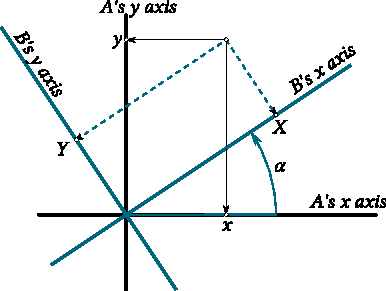
\includegraphics{01coordinatesRotated.pdf}
  \caption{After choosing different $x$ and $y$ axes, A and B will assign
    different $x, y$ coordinates to the same point in the plane.  Equations
    \eqref{eq:coordinateRotation} give the relation between these two sets of
    coordinates. }
  \label{fig:coordinateRotation}
\end{figure}

We are used to specifying the location of points in the plane by giving their
$x$ and $y$ coordinates, but sometimes it is better to use different
coordinates.  For instance, two people A and B could have chosen the same
origin, but their axes could be rotated with respect to each other. See
Figure~\ref{fig:coordinateRotation}.  If A's coordinates are called $x,y$ and
B's coordinates are $X,Y$ then it should be possible to find A's coordinates of
a point if we know what coordinates B assigns to this point -- given $X,Y$ what
are $x,y$?  The answer to this question is\footnote{One way of arriving at these
  relations is to use vectors as in the first vector work sheet of this
  semester.}
\begin{equation}\label{eq:coordinateRotation}
  \left\{
    \begin{aligned}
      x = X\cos\alpha - Y\sin\alpha,\\
      y = X\sin\alpha + Y\cos\alpha.
    \end{aligned}
  \right.
\end{equation}
Suppose both A and B are measuring the temperature $T$ at various points in the
plane.  A predicts the temperature at various points in the plane: he says that
at the point with coordinates $(x,y)$ the temperature will be $T(x, y)$.  In
fact he has also found the partial derivatives $\pdd {T}x $ and $\pdd {T}y $.

Equipped with the $X,Y \to x,y$ conversion \eqref{eq:coordinateRotation} B can
now take A's formula for the temperature and express it in terms of her own
$X,Y$ coordinates.  If we write $T_A(x, y)$ for the temperature at the point
whose A-coordinates are $(x,y)$ and $T_B(X,Y)$ for the temperature at the point
whose B-coordinates are $(X,Y)$, then we have
\begin{align*}
  T_B(X,&Y) = T_A(x,y)\\
  &= T_A(X\cos\alpha - Y\sin\alpha, X\sin\alpha + Y\cos\alpha).
\end{align*}
What is the relation between the partial derivatives of the temperatures as
computed by A and by B?  The chain rule gives the answer:
\begin{align*}
  \frac{\pd T_B}{\pd X} &= \pdd{}X\Bigl\{ T_A\bigl(\underbrace{X\cos\alpha -
    Y\sin\alpha}_{=x},
  \underbrace{X\sin\alpha + Y\cos\alpha}_{=y} \bigr)\Bigr\}\\
  &= \frac{\pd T_A}{\pd x} \cos\alpha + \frac{\pd T_A}{\pd y}\sin\alpha.
\end{align*}
\subsection{Another example -- Polar coordinates}
\label{sec:Chain-rule-polar-coordinates}
Suppose a quantity $P$ is given in terms of Cartesian coordinates $x$ and $y$:
$P=f(x, y)$.  How does $P$ change if we vary the polar coordinates $r$ and
$\theta$, i.e.\ what are the partial derivatives of $P$ with respect to $r$ and
$\theta$?

To answer this question we must write $P$ as a function of $r$ and $\theta$.
Recall that the relation between Cartesian coordinates and polar coordinates is
\begin{equation}\label{eq:polar-to-cartesian}
  x = r\cos \theta, \qquad y= r\sin \theta.
\end{equation}
Therefore $P=f(x, y) = f(r\cos \theta, r\sin \theta)$ and we get
\begin{equation}
  \pdd Pr = \cos \theta \pdd fx + \sin \theta \pdd fy,
  \qquad
  \pdd P \theta = 
  -r\sin \theta\pdd fx + r\cos \theta \pdd fy
\end{equation}
Since the function $f$ always gives us the value of the quantity $P$, these
relations are usually written in this way:
\begin{equation}
  \pdd Pr = \cos \theta \pdd Px + \sin \theta \pdd Py,
  \qquad
  \pdd P \theta = 
  -r\sin \theta\pdd Px + r\cos \theta \pdd Py
\end{equation}
Using the relation \eqref{eq:polar-to-cartesian} between polar and Cartesian
coordinates we can write these equations in yet another way:
\begin{equation}
  \pdd Pr = \frac xr \pdd Px + \frac yr \pdd Py,
  \qquad
  \pdd P \theta = -y \pdd Px + x \pdd Py
\end{equation}

 

\section{Problems}
\begin{multicols}{2}
\problemfont


\problem Use the chain rule to compute $dz/dt$ for 
$z=\sin(x^2+y^2)$, $x=t^2+3$, $y=t^3$.
\answer
$4xt\cos(x^2+y^2)+6yt^2\cos(x^2+y^2)$
\endanswer

\problem Use the chain rule to compute $dz/dt$ for 
$z=x^2y$, $x=\sin(t)$, $y=t^2+1$.
\answer
$2xy\cos t+2x^2t$
\endanswer

\problem Use the chain rule to compute $\partial z/\partial s$ and  
$\partial z/\partial t$ for
$z=x^2y$, $x=\sin(st)$, $y=t^2+s^2$.
\answer
$2xyt\cos(st)+2x^2s$, $2xys\cos(st)+2x^2t$
\endanswer

\problem Use the chain rule to compute $\partial z/\partial s$ and  
$\partial z/\partial t$ for
$z=x^2y^2$, $x=st$, $y=t^2-s^2$.
\answer
$2xy^2t-4yx^2s$, $2xy^2s+4yx^2t$
\endanswer


\problem\subprob Let $x=x(u,v), y=y(u,v)$ be  the following set of
functions of $u, v$:
\[
x=u^2-v^2,\quad y=2uv.
\]
If $g(u,v) = f(x(u,v), y(u,v))$ then compute $g_u(1,0)$,
$g_u(1,1)$, $g_v(1,0)$, and $g_v(1,1)$, if you are given these values
of the partial derivatives of $f$:

\begin{center}
  \begin{tabular}{cc|cc}
    $x$  & $y$  & $f_x(x, y)$ & $f_y(x, y)$ \\  \hline
    0 & 0 & $A$ & $B$\\
    1 & 0 & $C$ & $D$\\
    0 & 1 & $E$ & $F$\\
    1 & 1 & $G$ & $H$\\
    2 & 0 & $I$ & $J$\\
    0 & 2 & $K$ & $L$
  \end{tabular}
\end{center}

\subprob Repeat the above problem if $x$ and $y$ are given by $x=u$, $y=v/u$.

\subprob Repeat part \textbf{(a)} of this problem if $x$ and $y$ are given by $x=u+v$, $y=u-v$.

\problem Let $x, y, X, Y, T_A$, and $T_B$ be as in the example in 
\S\ref{sec:01rotated-coordinates}.  In that section we computed
$\pdd{T_B}X$.  

\subprob Compute $\DS\pdd{T_B}{Y}$.
\answer
$\pdd{T_B}{Y} = -\sin\alpha \pdd{T_A}{x} + \cos\alpha \pdd {T_A}{y}$.
\endanswer

\subprob Show that 
\[
\bigl(\pdd{T_A}x\bigr)^2+
\bigl(\pdd{T_A}y\bigr)^2=
\bigl(\pdd{T_B}X\bigr)^2+
\bigl(\pdd{T_B}Y\bigr)^2.
\]
In other words, A and B may measure different partial derivatives, but
the temperature gradients they find have the same length.
$\|\nab T_A\| = \|\nab T_B\|$.
\answer
Take the formulas for $\pdd{T_B}X$ and $\pdd{T_B}Y$ and work out the
right hand side in this problem.
\endanswer

\problem (About polar coordinates). In \S\ref{sec:Chain-rule-polar-coordinates} we saw how we can use the chain rule to find $\pdd fr$ and $\pdd f\theta$ if we know the function $f$ in terms of Cartesian coordinates $(x,y)$.  In this problem we turn the question around: suppose we are given a function in polar
coordinates, how do we compute its gradient.

Recall that polar and Cartesian coordinates are related by
\[
r=\sqrt{x^2+y^2}
\text{ and }
\theta = \arctan \frac yx,
\]
at least in the region where $x>0$. (See Chapter III, \S~\ref{sec:functions-in-PC}.)

\subprob Compute $\pdd rx$, $\pdd ry$, $\pdd\theta x$, $\pdd\theta y$.
Try to simplify your answer as much as possible, by reusing the
variables $r$ and $\theta$.  For instance, the simplest way to write
$\pdd rx$ is as $\pdd rx= \frac{x} {r}$.


\subprob Suppose a quantity $P$ is given in terms of Polar coordinates
by $P= f(r, \theta)$.  Express $\pdd Px$ and $\pdd Py$ in terms of
$\pdd fr$ and $\pdd f\theta$.  

More precisely, compute
\[
 \pdd Px \stackrel{\sf def}= \pdd {\bigl\{f(r(x,y), \theta(x,y)\bigr\}} {x}
\]
and
\[
 \pdd Py \stackrel{\sf def}= \pdd {\bigl\{f(r(x,y), \theta(x,y)\bigr\}} {y}
\]

\subprob Show that
\[
\|\nab P\|^2 = \bigl(\pdd fr\bigr)^2 + \frac{1} {r^2}\bigl(\pdd f\theta\bigr)^2.
\]

\problem For some function $f$ we are told that at the point 
with Cartesian coordinates $(4,3)$ one has 
\[
\pdd fr = 3, \quad \pdd f\theta = 6.
\]
Compute the gradient $\nab f$ at $(2,1)$.

\problem In physics an electric field is described by its \emph{potential 
  function}, $\phi=\phi(x,y)$ (in this problem we assume the world is
two-dimensional; the potential $\phi$ is measured in Volts).  Minus the
gradient of the potential function is called the \emph{electric field:}
\[
\vE = - \nab \phi.
\]
The electric potential of a point charge in the plane is given in Polar
coordinates by $\phi = -C\ln r$, for some constant $C$ (the physicists will
tell you that $C$ depends on the charge that was placed at the origin; for
us it is just some number, and we will in fact assume that $C=1$.)

\subprob Compute the electric field $\vE$ corresponding to the potential $\phi
= -\ln r$.
\answer $\vE = -\nab \ln r = \frac{1} {r^2}\tvek x\\ y\ttor$.
\endanswer

\subprob Compute $\| \vE\|$ (this quantity measures the strength of the
electric field, but not its direction.)  Where is the electric field
stronger?
\answer $\|\vE\| = 1/r = \frac{1} {\sqrt{x^2+y^2}}$.
\endanswer

\subprob Make a drawing of the level curves of the potential $\phi$, and the
electric field $\vE$.  

\subprob In the three dimensional world the electric potential generated by
a charged particle at the origin is not given by $-C\ln r$, but instead by
the so-called \textit{Coulomb potential}
\[
\phi = \frac{C} {r}, \text{ where } r= \sqrt{x^2+y^2+z^2}.
\]
Compute the corresponding electric field $\vE = -\nab \phi$.

\problem The {\em ideal gas law\/}, given by $PV=nRT$, relates the 
Pressure, Volume, and Temperature of $n$ moles of gas.  ($R$ is the
ideal gas constant).  Thus, we can view pressure, volume, and
temperature as variables, each one dependent on the other two.

(In this problem pressure is measured in Pascals, temperature in degrees
Kelvin, and volume in Liters.)

Each of the following three questions can be answered by applying the
chain rule to differentiate $z(t) = f(x(t), y(t))$ for suitable
quantities  $x$, $y$, and $z$.  In each case state which variables
play the role of $x, y, z$, and what the function $f$ is.

\subprob If pressure of a gas is increasing at a rate of $0.2
\text{Pa}/\text{min}$ and temperature is increasing at a rate of $1
^\circ\text{K}/\text{min}$, how fast is the volume changing?

\subprob If the volume of a gas is decreasing at a rate of $0.3
\text{L}/\text{min}$ and temperature is increasing at a rate of $0.5^\circ
\text{K}/\text{min}$, how fast is the pressure changing?

\subprob If the pressure of a gas is decreasing at a rate of $0.4
\text{Pa}/\text{min}$ and the volume is increasing at a rate of $3
\text{L}/\text{min}$, how fast is the temperature changing?

\problem The ideal gas law says $PV=nRT$, where $P,V,T$ are variables, 
and $n$, $R$ are constants.  Verify the following identity: 
\[
  {\partial P\over \partial V} {\partial V\over \partial T}
{\partial T\over \partial P}=-1
\]

\problem The previous exercise was a special case of the following 
fact, which you are asked to verify here:

Assume that $F(x,y,z)$ is a function of 3 variables, and suppose that
the relation $F(x,y,z)=0$ defines each of the variables in terms of
the other two, namely $x=f(y,z)$, $y=g(x,z)$ and $z=h(x,y)$, then
\[
\pdd xy \pdd yz \pdd zx =-1.
\]
Hint: this is a problem about implicit differentiation.


\problem
Four cartographers are using different coordinates to describe the
same landscape.  Each of them describes the landscape by specifying a
the height of a point in the landscape as a function of its position
above a horizontal plane.

Cartographer A uses Cartesian coordinates $(x, y)$ in the plane, B
uses Cartesian coordinates $(X,Y)$ in the plane.
The coordinates $(X,Y)$ are rotated by $45^\circ$ with respect to 
$(x, y)$ (see \S\ref{sec:01rotated-coordinates}).  

Cartographer C works with A but uses polar coordinates $(r, \theta)$
($r$ is the distance to the origin, $\theta$ is the angle with A's
$x$-axis).  

Cartographer D works with B and uses polar coordinates $(r, \varphi)$ 
($r$ is the distance to the origin, $\varphi$ is the angle with B's
$X$-axis).  

Here is a picture of the landscape that A, B, C, and D are
looking at:

\begin{center}
  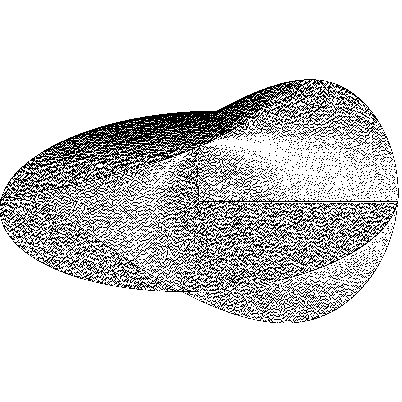
\includegraphics[width=0.3\textwidth]{01disco.pdf}
\end{center}

\subprob If B has found that the height is given by the function 
$f(X, Y) = 2XY/(X^2+Y^2)$, then what function does A find for the
height?
\answer
Height $ = - (x^2-y^2)/(x^2+y^2)$
\endanswer

\subprob What height function does C find?
\answer
Height $ = \sin 2\theta$.
\endanswer

\subprob What height function does D find?
\answer
Height $ = \cos 2\varphi$.
\endanswer

\problem Brian and Ally are using different Cartesian coordinate 
systems in the plane: $(x, y)$ for Ally, $(X,Y)$ for Brian.  They have
the same origin, but Brian's coordinates are rotated by an angle of
$\theta = \arctan \frac43$ ($\approx 53^\circ$, although that is only an
approximation.  You can give exact answers in this problem, and you
don't need a calculator.)

\subprob What is the relation between $(x,y)$ and $(X, Y)$?

\subprob If Ally has found that $T_A(x,y) = 32+0.1y$, then what
formula $T_B(X,Y)$ will Brian use to describe the temperature?

\subprob On a different occasion Ally found that the temperature had
changed.  Now Ally measures the temperature and finds that at the
point with $x=1, y=1$ one has $T_A(1,1) = 35$, and also $\pdd {T_A}x =
0.05$ and $\pdd{T_A}y = 0.8$.  Which coordinates does Brian assign to
this point, which temperature $T_B$, and which derivatives $\pdd
{T_B}X$ and $\pdd{T_B}Y$ does Brian compute at this point?

[Hint: before you compute anything, find $\sin \theta$ and
$\cos\theta$;  also draw a right triangle one of whose acute angles is
$\theta$.]
\noproblemfont

\end{multicols}

\section{Higher Partials and Clairaut's Theorem}

\subsection{Higher partial derivatives}     
By definition
\begin{equation}
  \begin{aligned}
    \frac{\pd ^2 f}{\pd x^2} &= \frac{\DS\pd \bigl(\pdd fx \bigr)}{\pd x}&
    \frac{\pd ^2 f}{\pd x \pd y} &=
    \frac{\DS\pd \bigl(\pdd fy \bigr)}{\pd x}\\
    \frac{\pd ^2 f}{\pd y \pd x} &= \frac{\DS\pd \bigl(\pdd fx \bigr)}{\pd y}&
    \frac{\pd ^2 f}{\pd y^2} &= \frac{\DS\pd \bigl(\pdd fy \bigr)}{\pd y}
  \end{aligned}
  \label{eq:second-partials-defined}
\end{equation}
In subscript notation one writes these higher partial derivatives as follows:
\[
\begin{aligned}
  f_{xx}(x, y) &= \frac{\pd ^2 f}{\pd x^2}&
  f_{xy}(x, y) &= \frac{\pd^2 f}{\pd y \pd x}\\
  f_{yx}(x, y) &= \frac{\pd^2 f}{\pd x \pd y}& f_{yy}(x, y) &= \frac{\pd^2
    f}{\pd y^2}\;.
\end{aligned}
\]
\emph{Note the reversal in $xy$ order in the mixed partial derivatives!}

\subsection{Example} If $f(x, y) = x^2y+\cos xy$ then $ f_x = 2xy - y\sin xy, $
and hence
\begin{eqnarray*}
  f_{xx} & = &
  \frac{\pd (2xy-y\sin xy)}{\pd x}=
  2y - y^2\cos xy,
  \\
  f_{xy} & = &
  \frac{\pd (2xy-y\sin xy)}{\pd y}=
  2x - \sin xy -xy \cos xy.
\end{eqnarray*}
The other partial derivatives follow from $f_y = x^2 - x\sin xy$, and they are
\[
f_{yx} = 2x - \sin xy - xy\cos xy, \quad f_{yy} = -x^2 \cos xy.
\]
Every time we take a derivative, we can choose whether we differentiate with
respect to $x$ or $y$.  Differentiating once we have two possibilities,
differentiating twice we have $2\times2 = 4$ possibilities, etc.  That is why we
found four partial derivatives of second order in the above example.  But if we
look carefully, we also see that $f_{xy}$ and $f_{yx} $ are the same.  This is
no coincidence.

\subsection{Clairaut's Theorem -- mixed partials are equal}     
\label{thm:Clairaut}
\textit{If for a given function $f$ of two variables the mixed partial
  derivative $f_{xy}(x, y)$ exists for all $(x, y)$ in a neighborhood of a point
  $(a,b)$, and if this derivative is continuous at $(a, b)$, then the other
  mixed partial derivative $f_{yx}(a,b)$ also exists, and $f_{xy}(a, b) =
  f_{yx}(a,b)$.  }

So we normally don't have to worry about the order in which we take partial
derivatives.

\subsection{Proof of Clairaut's theorem} With some algebra we can show that the
definition of partial derivatives implies
\begin{multline}
  \label{eq:Clairaut1}
  \frac{\pd^2 f}{\pd x \pd y} = \\
  \lim_{\Delta x\to 0}\lim_{\Delta y\to 0}
  \frac{f(x+\Delta x, y+\Delta y) - f(x, y+\Delta y) - f(x+\Delta x, y) +
    f(x, y)} {\Delta x \Delta y}
\end{multline}
while
\begin{multline}
  \label{eq:Clairaut2}
  \frac{\pd^2 f}{\pd y \pd x} = \\
  \lim_{\Delta y\to 0}\lim_{\Delta x\to 0}
  \frac{f(x+\Delta x, y+\Delta y) - f(x, y+\Delta y) - f(x+\Delta x, y) +
    f(x, y)} {\Delta x \Delta y}
\end{multline}
So it's a matter of showing that one can switch the two limits.  We won't go
into the details here, but the hypothesis that $f_{xy}$ is continuous implies
that we are indeed allowed to switch the limits.

\section{Finding a function from its derivatives} 
\label{sec:finding-f-from-its-derivs}
We now look at integrating
the partial derivatives of a function, which looks out of place here (this being
a chapter on derivatives and not on integrals), but Clairaut's Theorem actually
turns out to play a role.

If we have the derivative $f'(x)$ of some function of one variable then we know
how to recover the function $f(x)$: we integrate, i.e.
\[
f(x) = \int f'(x) dx + C.
\]
Furthermore, any (continuous) function can be the derivative of a function,
because, if someone gives us a continuous function $f(x)$, then
\[
F(x) \stackrel{\rm def}{=} \int_a^x f(t) dt
\]
is a differentiable function whose derivative is $F'(x) = f(x)$.

What about functions of more than one variable?  Suppose we know the partial
derivatives
\begin{equation}\label{eq:potential}
  \pdd fx  = P(x, y) \text{ and }
  \pdd fy  = Q(x, y)
\end{equation}
of a function of two variables, can you then find the function $f(x,y)$?

The answer is ``yes, you can find $f$ by integrating, \emph{if it exists,} but not
every pair of functions $P$ and $Q$ are the partial derivatives of some function.''

The following two examples are typical of what can happen.


\subsection{Example}     
Does there exist a function $f(x, y)$ of two variables such that
\[
\pdd fx = x^3 - 2xy,\text{ and } \pdd fy = 3y^2
\]
both hold?  The answer is no, such a function cannot exist, and here is the
reason: if there were such a function, then we could compute
\[
\frac{\pd^2 f}{\pd y \pd x} = \frac{\pd( x^3 - 2xy)}{\pd y} = -2x, \text { and }
\frac{\pd^2 f}{\pd x \pd y} = \frac{\pd (3y^2)}{\pd x} = 0.
\]
By Clairaut's Theorem both computations should give us the same answer, but they
don't.  Therefore the function $f$ whose partials are as above cannot exist.

\subsection{Example}     
Does there exist a function $f(x, y)$ of two variables whose derivatives are
\[
\pdd fx = x^3 - 2xy,\text{ and } \pdd fy = \sin \pi y - x^2 ?
\]
Let's check Clairaut's condition:
\[
\frac{\pd^2 f}{\pd y \pd x} = \frac{\pd( x^3 - 2xy)}{\pd y} = -2x, \text { and }
\frac{\pd^2 f}{\pd x \pd y} = \frac{\pd (\sin \pi y - x^2)}{\pd x} = -2x.
\]
This time both computations gave us the same answer, so Clairaut's theorem does
not rule out the existence of the function $f$ that we are looking for.  We can
try to compute it by integrating both partial derivatives.  There is a
systematic way of doing this that usually leads to the answer.

We first integrate $f_x$ while treating $y$ as a constant:
\[
f(x, y ) = \int \{x^3-2xy\} \; dx = \tfrac14 x^4 - x^2y + C(y).
\]
The ``constant'' is only a constant in the sense that it does not depend on $x$.
It may depend on $y$, and that is why we wrote it as $C(y)$.  To find $C(y)$ we
differentiate this result with respect to $y$:
\[
\sin\pi y - x^2 = f_y = \frac{\pd \bigl\{ \tfrac14 x^4 - x^2y + C(y)\bigr\}
}{\pd y} = -x^2 + C'(y).
\]
So we see that $C'(y) = \sin\pi y$, and hence $C(y) = -\frac1\pi \cos\pi y + K$,
where $K$ is a real constant ($K$ depends neither on $x$ nor on $y$).

We find that the following function has the prescribed partial derivatives
\[
f(x, y) = \tfrac14 x^4 - x^2y -\tfrac1\pi \cos \pi y + K
\]
where $K$ is constant, i.e.~where $K$ depends on neither $x$ nor $y$.

The method used in this example always works, and we summarize this fact in the
following theorem.
\begin{theorem} Suppose $P(x, y)$ and $Q(x,y)$ are two functions that are
  defined on a rectangular domain $\cR = \{(x, y) : a<x<b, c<y<d\}$, and suppose
  that they have continuous partial derivatives on this domain.

  If a function $f(x, y)$ exists such that \eqref{eq:potential} holds on $\cR$,
  then
  \begin{equation}\label{eq:exact}
    \pdd Py = \pdd Qx
  \end{equation}
  must hold on $\cR$.

  Conversely, if $P$ and $Q$ satisfy \eqref{eq:exact} then there is a function
  $f$ defined on $\cR$ that satisfies \eqref {eq:potential}.
\end{theorem}

\bigskip

To prove this theorem we need to understand integrals of functions of several
variables, and Green's theorem in particular, so this will have to wait until
the end of the semester.  See \S~VII.\ref{sec:clairaut-is-conservative}.

It should be noted that the assumption above that the functions $P$ and $Q$ be
defined on a rectangle is important: the theorem is no longer true if the domain
of $P$ and $Q$ ``has holes.''  See problem \ref{prb:grad-of-theta}.

\newpage
\section{Problems}
\label{sec:partial-deriv-problems}
\begin{multicols}{2}
\problemfont 
\problem Find all first and second partial derivatives of $x^3y^2+y^5$.  
\answer $f_x=3x^2y^2$, $f_y=2x^3y+5y^4$, $f_{xx}=6xy^2$,
$f_{yy}=2x^3+20y^3$, $f_{xy}=6x^2y$
\endanswer

\problem Find all first and second partial derivatives of $4x^3+xy^2+10$.  
\answer
$f_x=12x^2+y^2$, $f_y=2xy$, $f_{xx}=24x$, $f_{yy}=2x$, $f_{xy}=2y$
\endanswer

\problem Find all first and second partial derivatives of $x\sin y$.  
\answer $f_x=\sin y$, $f_y=x\cos y$, $f_{xx}=0$, $f_{yy}=-x\sin y$,
$f_{xy}=\cos y$
\endanswer

\problem Find all first and second partial derivatives of  
$\sin(3x)\cos(2y)$.

\problem Find all first and second partial derivatives of $e^{x+y^2}$.  

\problem Find all first and second partial derivatives of  
$\ln\sqrt{x^3+y^4}$.

\problem Find all first and second partial derivatives of $z$ with respect  
to $x$ and $y$ if $x^2+4y^2+16z^2-64=0$.  (Hint: solve for $z$ or use implicit
differentiation\ldots)

\problem Find all first and second partial derivatives of $z$ with respect  
to $x$ and $y$ if $xy+yz+xz=1$. (Hint: solve for $z$ or use implicit
differentiation\ldots)

\problem How many different second partial derivatives does a function of  
two variables have?  What about a function of three variables?  How many
derivatives of third degree does a function of two variables have?
\answer
A function of two variables has
\[
  f_{xx},\qquad f_{xy}=f_{yx},\qquad f_{yy},
\]
so it has \emph{three} different partial derivatives of second order.

A function of three variables has these partial derivatives:
\[
  \begin{matrix}
    f_{xx} & f_{xy} & f_{xz} \\
    f_{yx} & f_{yy} & f_{yz} \\
    f_{zx} & f_{zy} & f_{zz}
  \end{matrix}
\]
The ones ``below the diagonal'' are the same as corresponding derivatives
above the diagonal, so there are only six different partial derivatives
of second order, namely these:
\[
  \begin{matrix}
    f_{xx} & f_{xy} & f_{xz} \\
    & f_{yy} & f_{yz} \\
    & & f_{zz}
  \end{matrix}
\]
A function of two variables has 
\begin{gather*}
  f_{xxx}, \\
  f_{xxy}=f_{xyx}=f_{yxx}, \\
  f_{xyy}=f_{yxy}=f_{yyx},\\
  \text{ and } f_{yyy}
\end{gather*}
so \emph{four} different partial derivatives of third order.
\endanswer

\problem Derive the formulas \eqref{eq:Clairaut1} and  
\eqref{eq:Clairaut2} from the definition of partial derivatives
\eqref{eq:partial-wrt-x-defined} and
\eqref{eq:partial-wrt-y-defined}.

\problem The equation which describes the \textit{vibrating  string}  
(as in a guitar, piano, or violin string) is
\begin{equation}\label{eq:wave-equation}
  \frac{\partial^2 f}{\partial t^2} = c^2 \frac{\partial^2 f}{\partial x^2}
\end{equation}
where $c>0$ is some constant. The equation is called the \emph{wave
equation}.  It is an example of a \emph{partial differential equation.}

Note : this problem looks like a problem about differential
equations, but to answer the following questions you really only have
to compute partial derivatives of certain functions, and solve some
(easy) algebraic equations.

\subprob For which values of the constant $v$ is a ``traveling wave
with velocity $v$ and profile $F(x)$'' a solution of the wave equation
\eqref{eq:wave-equation}?  In other words, for which values of the constant $v$ is the function
\[
f(x, t) = F(x-vt)
\]
a solution of \eqref{eq:wave-equation}?

Does it matter which profile $F$ is used
here?

(For the terminology used here, revisit problem
\ref{prb:01traveling-waves} in Chapter III, \S\ref{sec:graphing-problems-2d3d}.)

\subprob Suppose the string is clamped down at its ends, and that its
length is $L$.  For which values of the constants $A$ and $\alpha$ is
\[
  f(x, t) = A\sin(\alpha t) \sin \frac{\pi x}{L}
\]
a solution of the wave equation?  (Assume $A\neq0$).

\subprob Same question for 
\[
  g(x, t) =  B\sin(\beta t) \sin \frac{2\pi x}{L}.
\]
\subprob Describe the movies that go with the solutions you found in \textbf{(b)} and \textbf{(c)}.  Which of the two graphs moves faster?

\subprob Show that $h(x, t) = f(x, t)+g(x, t)$ is again a solution of the
wave equation, where $f$ and $g$ are as above.  (Don't use the formulas for
$f$ and $g$: it is easier to prove a more general fact, namely, if two
functions $f$ and $g$ satisfy (\ref{eq:wave-equation}), then so does their
sum $f+g$.)


\subprob Describe the movie that goes with the function $h(x,t)$ (it is probably better to use a graphing application like \texttt{grapher.app} on Mac OS X,
\texttt{graphcalc.exe} on Windows or Linux).

\problem Suppose $P(x, y) = x^2-2xy^3$ and $Q(x, y) = (xy)^2$.  Does  
there exist a function $f(x, y)$ such that $P= f_x$ and $Q= f_y$?

\problem Suppose $P(x, y) = x^2+axy^3$ and $Q(x, y) = (xy)^2$, where $a$  
is a constant.  For which $a$ does there exist a function $f(x, y)$ such
that $P= f_x$ and $Q= f_y$?

\problem
\subprob Does there exist a function $f(x, y)$ such that
\[
f_x = ax^2y + bxy^2, \quad f_y = y^3+x^3\;?
\]
where $a,b$ are constants.
\answer
Clairaut requires $f_{xy} = f_{yx}$, which leads to $a=3$, $b=0$.  So there is no solution unless $a=3$ and $b=0$.  \emph{If} $a=3$ and $b=0$ then the solution is $f(x,y) = x^3y + \frac14 y^4 $.
\endanswer

\subprob
Does there exist a function $f(x, y)$ such that
\begin{align*}
f_x &= ax^2y + bxy^2+k\cos x, \\
f_y &= y^3+x^3-l e^y\;?
\end{align*}
where $a, b, k, l$ are constants.
\answer
Again, there is no solution unless $a=3$ and $b=0$.  There is no restriction on $k$ $or l$.  \emph{If} $a=3$ and $b=0$ then the solution is $f(x,y) = x^3y + \frac14 y^4 + k\sin x - le^y$.
\endanswer

\problem Suppose $x=u+v$, $y=u-v$, and suppose $f(x, y) = g(u, v)$.  
Then compute

\subprob $\dfrac{\pd^2 g}{\pd u^2}$%
\answer
We have $g(u,v) = f(u+v, u-v)$, so
\[
  \pdd gu = \pdd fx \pdd{(u+v)}u + \pdd fy \pdd{(u-v)}u
  = f_x(u+v, u-v)+f_y(u+v, u-v).
\]
Similarly,
\[
  \pdd gv = f_x(u+v, u-v) - f_y(u+v, u-v).
\]
Differentiate again to get
\(\DS
  \frac{\pd^2 g}{\pd u^2}
  = f_{xx}(u+v, u-v)+2f_{xy}(u+v, u-v)+f_{yy}(u+v, u-v).
\)
\endanswer

\subprob $\dfrac{\pd^2 g}{\pd v^2}$
\answer
\(\DS 
\frac{\pd^2 g}{\pd v^2}
= f_{xx}(u+v, u-v)-2f_{xy}(u+v, u-v)+f_{yy}(u+v, u-v)
\)

Note that this is almost the same as $\dfrac{\pd^2g}{\pd u^2}$: the only change is in the minus sign before $f_{xy}$.
\endanswer

\subprob   $\dfrac{\pd^2 g}{\pd u\pd v}$
\answer
   $\DS\frac{\pd^2 g}{\pd u\pd v}= f_{xx}(u+v, u-v) - f_{yy}(u+v, u-v)$
\endanswer

\subprob $\dfrac{\pd^2 g}{\pd u^2} - \dfrac{\pd^2 g}{\pd v^2}$
\answer
$\dfrac{\pd^2 g}{\pd u^2} - \dfrac{\pd^2 g}{\pd v^2} = 4f_{xy} $
\endanswer

\subprob $\dfrac{\pd^2 g}{\pd u^2} + \dfrac{\pd^2 g}{\pd v^2}$
\answer
$\dfrac{\pd^2 g}{\pd u^2} + \dfrac{\pd^2 g}{\pd v^2} = 2\bigl(f_{xx}+f_{yy}\bigr)$.
\endanswer

\problem\label{prb:grad-of-theta} 
[For discussion] Let 
\[
  P(x,y) = \frac{-y}{x^2+y^2},
  \quad
  Q(x,y) = \frac{x}{x^2+y^2}.
\]

\subprob What is the domain of $P$ and $Q$?

\subprob Show that
\[
  P = \pdd\theta x, \qquad
  Q = \pdd\theta y
\]
where $\theta$ is the angle variable from polar coordinates.

\subprob Show that $P$ and $Q$ satisfy the condition
(\ref{eq:exact}).  (You don't have to compute the derivatives to
check this, although you could.)

\subprob Is there a function $f$ such that (\ref{eq:potential}) holds?

\noproblemfont
\end{multicols}

%%% Local Variables: 
%%% mode: latex
%%% TeX-master: "free234"
%%% End: 
